\documentclass[journal]{IEEEtran}

% ===================== PACKAGES =====================
\usepackage{amsmath,amssymb,amsfonts}
\usepackage{amsthm}
\usepackage{algorithm}
\usepackage{algpseudocode}
\usepackage{array}
\usepackage{booktabs}
\usepackage{multirow}
\usepackage{makecell}
\usepackage{threeparttable}
\usepackage{graphicx}
\usepackage{xcolor}
\usepackage{tikz}
\usepackage{pgfplots}
\pgfplotsset{compat=1.18}
\usepgfplotslibrary{groupplots}
\usetikzlibrary{arrows.meta,positioning,shapes.geometric,fit,calc,backgrounds,automata,decorations.pathreplacing}
\usepackage{subcaption}
\usepackage[hidelinks]{hyperref}
\usepackage{url}

% ---- float placement tuning (two-column) ----
\renewcommand{\topfraction}{0.95}
\renewcommand{\bottomfraction}{0.95}
\renewcommand{\textfraction}{0.05}
\renewcommand{\floatpagefraction}{0.85}
\renewcommand{\dbltopfraction}{0.95}
\renewcommand{\dblfloatpagefraction}{0.85}
\setlength{\textfloatsep}{9pt plus 2pt minus 3pt}
\setlength{\floatsep}{9pt plus 2pt minus 3pt}
\setlength{\intextsep}{9pt plus 2pt minus 3pt}
\setlength{\dbltextfloatsep}{11pt plus 2pt minus 3pt}

% ---- colorblind-safe palette (Wong) ----
\definecolor{cbBlue}{HTML}{0072B2}
\definecolor{cbOrange}{HTML}{E69F00}
\definecolor{cbGreen}{HTML}{009E73}
\definecolor{cbRed}{HTML}{D55E00}
\definecolor{cbPurple}{HTML}{CC79A7}
\definecolor{cbCyan}{HTML}{56B4E9}
\definecolor{cbYellow}{HTML}{F0E442}
\definecolor{cbGray}{HTML}{555555}

% ---- theorem environments ----
\newtheorem{theorem}{Theorem}
\newtheorem{lemma}{Lemma}
\newtheorem{definition}{Definition}
\newtheorem{assumption}{Assumption}
\newtheorem{corollary}{Corollary}
\newtheorem{proposition}{Proposition}

\begin{document}

\title{SAGE: Zero-Halt Migration Between Heterogeneous Consensus Engines\\for Permissioned Blockchains}

% \author{Tuan-Dung~Tran and Nguyen~Thai~Cong
% \thanks{T.-D. Tran is with the University of Information Technology, Vietnam National University, Ho Chi Minh City, Vietnam (e-mail: dungtrt@uit.edu.vn).}%
% \thanks{Corresponding author: Tuan-Dung Tran.}}

% \markboth{Preprint, 2026}
% {Tran: Zero-Halt Migration Between Heterogeneous Consensus Engines}

\maketitle

\begin{abstract}
Permissioned and sovereign blockchains are routinely launched on a simple
Proof-of-Authority runtime and later need a high-throughput Byzantine fault tolerant
engine such as pipelined HotStuff. Replacing the consensus engine of a chain that is
already serving clients is a dependability problem rather than a module swap, because
state continuity, client interface stability, safety across the transition boundary, and
a safe abort path must all hold at once. Deployed systems already perform live
transitions, the Ethereum Merge ran a parallel beacon chain before a terminal-difficulty
cutover, and Polkadot, Cosmos, and Tezos perform on-chain upgrades, yet none of these
provides a formally proven, verifiable, and reversible transition between two structurally
different consensus engines. This paper presents SAGE, a migration protocol that keeps a
single finalizer during a bounded dual-run interval, gates cutover on a quorum-certified
decision over a stability predicate, binds the transition with a threshold-signed
migration manifest, and supports a deadline-bounded rollback. We prove uniqueness of the
cutover decision through quorum intersection, cross-boundary safety as an inductive
invariant, quantified zero-halt liveness that bounds the handoff warm-up, migration
termination, rollback correctness under a two-tier finality model, and manifest
unforgeability and replay resistance as cryptographic reductions. We evaluate SAGE along three complementary evidence tiers: a deterministic event-driven
simulator, a multi-process testbed of validators running as separate operating-system
processes over loopback TCP, and a bounded TLA+/TLC model check. The simulator
completes 30 no-partition migration seeds for each baseline and records mean SAGE
cutover-evidence latency of 105.2 microseconds in simulator time. Across the partition
matrix a disjoint-quorum exposure metric separates the strategies: under a cutover-straddling
balanced partition, hard fork and blind cutover are exposed to a fork window in every trial
while SAGE's certified cutover keeps exposure at zero. Because the serialized simulator cannot
realize a concurrent two-leader conflict, we additionally drive the real engines in the
multi-process testbed under an identical balanced partition at the cutover height: the
ungated control forks in every run while quorum-gated SAGE forks in none, so the
fork SAGE prevents is exhibited as a measured event rather than a structural impossibility.
A bounded model check exhaustively verifies cross-boundary safety, cutover-decision
uniqueness, and no-absolute-reversion over $n\in\{4,7,10\}$ and all partition splits, with
falsifying broken controls the checker must catch. The local runtime additionally exercises
SAGE cutover, post-cutover HotStuff finalization, store-backed double-vote rejection, and
restart/continue recovery from in-memory snapshots.
\end{abstract}

\begin{IEEEkeywords}
Consensus migration, Byzantine fault tolerance, HotStuff, Proof-of-Authority, permissioned
blockchain, live upgrade, state machine replication, quorum intersection, bounded
rollback, threshold signatures.
\end{IEEEkeywords}

% ===================== INTRODUCTION =====================
\section{Introduction}
\IEEEPARstart{N}{ational} and enterprise digital infrastructure increasingly relies on
permissioned blockchains that preserve a familiar execution model while satisfying
accountability, regulated access, and domestic integration constraints. A recurring
deployment pattern in this setting is staged. A network launches on a simple
Proof-of-Authority (PoA) runtime that is easy to operate and to audit, and only later,
once adoption and validator diversity grow, does it require a high-throughput Byzantine
fault tolerant (BFT) engine with deterministic sub-second finality. Sovereign deployments
make this pattern explicit because operators control the validator set and the upgrade
calendar, yet they cannot tolerate service interruption, client breakage, or any
ambiguity about which ledger state is canonical during an upgrade. The consensus engine is
therefore not a static design choice but a component that must itself be replaceable on a
running system, and the replacement must be safe, live, auditable, and reversible.

Modern BFT research has produced engines that are attractive migration targets.
Leader-based pipelined protocols such as HotStuff achieve linear communication and
responsiveness~\cite{hotstuff}, and directed acyclic graph designs such as Narwhal and
Tusk~\cite{narwhal}, Bullshark~\cite{bullshark}, Shoal~\cite{shoal},
Autobahn~\cite{autobahn}, and Mysticeti~\cite{mysticeti} raise throughput and lower
latency. Deployed systems have also performed live consensus transitions at scale. The
Ethereum Merge replaced Nakamoto proof of work with the Gasper proof-of-stake
protocol~\cite{gasper,casperffg} by running a parallel beacon chain for an extended period
and then cutting over at a terminal total difficulty. Polkadot performs forkless runtime
upgrades and finalizes with GRANDPA~\cite{grandpa}, the Cosmos software stack coordinates
in-protocol upgrades at a governed height, and Tezos amends its own protocol on chain,
including a change of its consensus algorithm to Tenderbake~\cite{tenderbake}. These
mechanisms demonstrate that live transitions are feasible and valuable, but each is a
mechanism-specific engineering artifact: none offers a general construction that takes a
chain from one consensus engine to a structurally different one with an explicit
cross-boundary safety argument and a verifiable way to undo the transition if it
goes wrong.

The specific open problem is a safe, live, and reversible transition between two
heterogeneous consensus engines on a running permissioned chain. A stop-the-world
migration halts the chain, snapshots state, and restarts under the new engine, which
produces measurable downtime and a finality gap. A flag-day hard fork coordinates a height
at which validators switch, which avoids a snapshot but risks a chain split if any
validator or network partition disagrees about the switch~\cite{tendermint,bitcoin}. Live
reconfiguration as formalized for state machine replication~\cite{reconfig,bftsmart} and
recently extended to a consensusless blockchain~\cite{suilutris} changes the validator set
safely but keeps a single fixed protocol, so it cannot by itself carry a chain from PoA to
a BFT engine, because the finalization rule itself changes. The Merge-style parallel run is
the closest deployed analogue, yet it provides neither a formal cross-boundary safety
theorem nor a bounded, verifiable rollback object, and it is specific to one protocol pair.
The gap, therefore, is not whether a live transition is possible, but whether it can be
made general, provably safe at the boundary, and verifiably reversible.

This paper addresses that gap with SAGE, a migration protocol built around four
mechanisms: a single-finalizer dual-run invariant, a quorum-certified cutover decision, a
threshold-signed migration manifest, and a deadline-bounded rollback under a two-tier
finality model. During a bounded dual-run interval the legacy engine remains the only
finalizer, so exactly one canonical chain exists, while the target engine validates that
identical chain in shadow mode and recomputes its own state roots. Cutover transfers
authority only when a quorum of validators jointly certifies a stability predicate over
consecutive shadow-valid blocks with matching roots, which makes the cutover a single
agreed decision rather than a set of independent local choices. A threshold-signed manifest
binds the boundary to a specific chain identifier, epoch, and parent so that an abort before
a fixed deadline returns the chain deterministically to the legacy state, and so that any
auditor can verify the transition after the fact. The main contributions are as follows.
\begin{enumerate}
  \item We formalize heterogeneous consensus migration through an abstract engine interface
  and a labeled transition system, define the shadow-anchoring invariant under which two
  engines coexist without ever both finalizing a block, and state the target consensus-state
  bootstrap that a heterogeneous handoff requires.
  \item We design SAGE with a quorum-certified cutover decision (a CutCert) and a
  threshold-signed migration manifest bound to chain identifier, epoch, and parent hash, and
  we give the controller as an explicit algorithm with constant per-block work and linear
  one-time decision cost.
  \item We prove uniqueness of the cutover decision through quorum intersection,
  cross-boundary safety as an inductive invariant, quantified zero-halt liveness that bounds
  the boundary warm-up, migration termination, and rollback correctness under a two-tier
  provisional and absolute finality model that reconciles reversibility with client
  semantics.
  \item We give cryptographic security games for manifest unforgeability and replay
  resistance with reductions to signature unforgeability and hash collision resistance, a
  detection-probability theorem that turns the shadow-anchoring ablation into a closed-form
  bound, and message and round complexity theorems for cutover and abort.
  \item We evaluate SAGE with deterministic simulator campaigns, a
  multi-process testbed, a bounded model check, and a one-process local runtime. The
  evaluation reports no observed safety violations in the simulator partition
  model, an observed cross-boundary fork differential in the multi-process testbed in which the
  ungated control forks in every run while quorum-gated SAGE never forks, exhaustive model-check
  verification of the boundary-safety and rollback invariants over $n\in\{4,7,10\}$, SAGE
  cutover-evidence latency and validator-count scaling, in-window rollback and past-deadline
  reversion refusal, and restart/continue recovery in the local runtime.
\end{enumerate}

The remainder of this paper is organized as follows. Section~\ref{sec:related} reviews
related work, including deployed live transitions, and positions SAGE.
Section~\ref{sec:model} states the system model, the abstract engine interface, and the
combined fault threshold. Section~\ref{sec:threat} gives the threat model and the abort
trigger analysis. Section~\ref{sec:protocol} presents the SAGE protocol and the
cryptographic manifest. Section~\ref{sec:analysis} proves the safety, liveness,
termination, rollback, and cryptographic properties and analyzes complexity.
Section~\ref{sec:eval} reports the experimental evaluation. Section~\ref{sec:discussion}
discusses generality, deployment, and limitations, and Section~\ref{sec:conclusion}
concludes.

% ===================== RELATED WORK =====================
\section{Related Work}
\label{sec:related}

\subsection{Byzantine Fault Tolerant Consensus}
The theory of agreement under failures establishes the impossibility of deterministic
consensus with a single faulty process in fully asynchronous networks~\cite{flp} and the
feasibility of agreement under partial synchrony~\cite{dls}. Practical Byzantine fault
tolerance~\cite{pbft} brought these ideas to deployable systems, and crash-tolerant
protocols such as Paxos~\cite{paxos} and Raft~\cite{raft} shaped the engineering of
replicated logs. Blockchain demand revived the area. HotStuff~\cite{hotstuff} achieves
linear message complexity and responsiveness through pipelining, Tendermint~\cite{tendermint}
popularized a gossip-based BFT for chains, and a family of directed acyclic graph protocols,
including Narwhal and Tusk~\cite{narwhal}, Bullshark~\cite{bullshark}, Shoal~\cite{shoal},
Autobahn~\cite{autobahn}, and Mysticeti~\cite{mysticeti}, separates dissemination from
ordering to raise throughput. This body of work defines candidate target engines for a
migration but assumes the consensus protocol is fixed once a chain is running, which is the
assumption we relax. Flexible BFT~\cite{flexbft} is closest in spirit on heterogeneous
assumptions: it lets clients with different beliefs draw different commit decisions from one
transcript. SAGE differs in that the two engines are temporally sequenced rather than
simultaneously interpreted, and the boundary between them is the object that must be made
safe.

\subsection{Live Protocol Transitions in Deployed Systems}
The most prominent real-world precedents for SAGE are industrial. The Ethereum Merge
replaced a Nakamoto proof-of-work engine with the Gasper proof-of-stake
protocol~\cite{gasper}, which couples the Casper finality gadget~\cite{casperffg} with a
fork-choice rule. Operationally the transition ran a separate beacon chain in parallel for
an extended period and then cut over when a terminal total difficulty was reached. This is a
shadow-then-cutover pattern and the closest deployed analogue to our dual-run and cutover,
but it was engineered for one specific pair of protocols, it provides no formal
cross-boundary safety theorem, and it offers no bounded, verifiable rollback once the cutover
has occurred. Polkadot performs forkless runtime upgrades and obtains finality from the
GRANDPA gadget~\cite{grandpa}, which finalizes chains rather than blocks and informs clients
when commits are still provisional, a design that resonates with our two-tier finality model.
The Cosmos stack coordinates in-protocol upgrades at a governance-scheduled height, and Tezos
amends its protocol on chain, including a transition of its consensus algorithm to
Tenderbake~\cite{tenderbake}, a dynamic repeated-consensus protocol with deterministic
finality and evolving committees. These systems show that live upgrades are practical and
valuable; what they do not provide, and what SAGE contributes, is a general construction with
an explicit cross-boundary safety argument, an executable invariant monitor that checks it on
every simulated run, and a manifest-bound, deadline-limited rollback.

\subsection{Reconfiguration, Forks, and Membership Change}
Changing a running replicated system has been studied mainly as membership reconfiguration.
Lamport, Malkhi, and Zhou formalize reconfiguration of a state machine~\cite{reconfig}, and
BFT-SMaRt~\cite{bftsmart} implements reconfiguration for Byzantine replication while keeping
one protocol. Sui Lutris~\cite{suilutris} gives a provably safe reconfiguration protocol for a
consensusless blockchain and reports no visible performance degradation across reconfiguration
events, which is the closest academic result to ours in rigor. The crucial distinction is that
reconfiguration changes which validators run a fixed protocol, so the finalization rule, the
quorum structure, and the certificate format are invariant across the change. SAGE changes the
protocol the validators run, which alters the finalization rule itself, so the standard
configuration-object abstraction does not apply and a dedicated cross-boundary argument is
required. The cutover decision is itself a one-shot agreement, which connects SAGE to the
literature on view synchronization and pacemakers for leader-based BFT: the readiness gather and
CutCert play a role analogous to a synchronizer that brings correct validators into a common
view before the target engine takes over. In the public-chain setting, protocol changes are
usually deployed as hard forks coordinated at a flag-day height~\cite{tendermint,bitcoin}, an
approach that trades a snapshot for the risk of a chain split when validators or network
partitions disagree about the switch; our evaluation reproduces exactly this failure as an
emergent behavior.

\subsection{Runtime Consensus-Protocol Switching}
The work closest to SAGE switches the consensus protocol itself at runtime rather than the
validator set. The ``Abstract'' framework and its Aliph instantiation~\cite{abstract} compose a
BFT protocol from abortable state-machine-replication instances and switch to the next instance
when the current one aborts, with a composability theorem that preserves total order across
switches. Cox~\cite{cox} makes the live switch concrete and engine-agnostic, hot-swapping a
running BFT engine (demonstrated PBFT$\leftrightarrow$HotStuff) with no downtime: it triggers on
a configuration block, certifies epoch termination with a threshold-aggregated
\emph{StableCheckpoint} that is structurally analogous to our CutCert, and recovers lagging nodes
through an epoch-mismatch sub-protocol. We therefore do not claim that live consensus switching
is itself new. SAGE differs along three axes that none of this prior work addresses jointly.
First, Abstract and Cox switch among \emph{homogeneous} engines that share one fault model and
quorum family (Byzantine $\leftrightarrow$ Byzantine); SAGE crosses fault models and finalization
rules (authority/crash-style PoA $\rightarrow$ Byzantine BFT), where the quorum structure and
certificate format themselves change at the boundary. This heterogeneous crossing, rather than
live switching as such, is the distinguishing problem SAGE addresses. Second, like Abstract and
Cox we give a pen-and-paper safety argument; we do not claim a mechanized proof, but we pair the
argument with an executable invariant monitor (Section~\ref{sec:eval}) that checks the
cross-boundary properties on every simulated run, which neither Abstract nor Cox reports. Machine
checked safety for a live change has so far been demonstrated only for \emph{reconfiguration} of a
fixed protocol~\cite{mongoraft,suilutris}, never for an engine boundary, and we leave a mechanized
boundary proof as future work. Third, Cox provides only forward catch-up recovery and Abstract
instances abort forward; neither offers a manifest-bound, deadline-limited verifiable rollback of
the transition, which SAGE makes a first-class mechanism.

\subsection{Permissioned and Sovereign Infrastructure}
Permissioned platforms emphasize known validators, modular ordering, and operational
accountability. Hyperledger Fabric~\cite{fabric} treats the ordering service as pluggable and
integrates identity-based membership, and execution-layer advances such as
Block-STM~\cite{blockstm} show that high throughput depends on the whole stack, not consensus
alone. Sovereign deployments add national identity, regulated finance, and a controlled
upgrade calendar, and post-quantum readiness is increasingly a requirement following the
standardization of lattice-based primitives~\cite{nistpqc}. These platforms motivate staged
consensus deployment but leave the engine transition itself unspecified, which is the gap
SAGE fills.

\begin{table}[t]
\centering
\caption{Comparison of approaches to changing a live replicated or blockchain system.
``Protocol swap'' replaces the consensus engine with a structurally different one;
``Verif.\ rollback'' is a cryptographically verifiable, bounded undo of the transition.
Runtime-swap (Cox)~\cite{cox} is the closest prior work but switches \emph{homogeneous}
BFT engines; $\dagger$ marks that SAGE's swap is additionally \emph{heterogeneous}, crossing
fault model and finalization rule, and is the only entry carrying a verifiable bounded
rollback.}
\label{tab:related}
\setlength{\tabcolsep}{3pt}
\renewcommand{\arraystretch}{1.18}
\footnotesize
\begin{tabular}{lccccc}
\toprule
Approach & \makecell{Zero\\halt} & \makecell{Protocol\\swap} & \makecell{Fork\\safe} & \makecell{Verif.\\rollback} & \makecell{Client\\stable} \\
\midrule
Stop-the-world~\cite{reconfig}         & \texttimes & \checkmark & \checkmark & \texttimes & \texttimes \\
Hard-fork flag-day~\cite{tendermint}   & \checkmark & \checkmark & \texttimes & \texttimes & \texttimes \\
Ethereum Merge~\cite{gasper}           & \checkmark & \checkmark & \checkmark & \texttimes & \texttimes \\
Forkless upgrade~\cite{grandpa}        & \checkmark & partial    & \checkmark & \texttimes & \checkmark \\
Cosmos x/upgrade~\cite{tenderbake}     & \texttimes & \texttimes & partial    & \texttimes & partial \\
Runtime swap (Cox)~\cite{cox}          & \checkmark & \checkmark & \checkmark & \texttimes & \checkmark \\
SMR reconfig~\cite{bftsmart}           & \checkmark & \texttimes & \checkmark & \texttimes & \checkmark \\
Sui Lutris reconfig~\cite{suilutris}   & \checkmark & \texttimes & \checkmark & \texttimes & \checkmark \\
\textbf{SAGE (this work)}              & \checkmark & \checkmark$^\dagger$ & \checkmark & \checkmark & \checkmark \\
\bottomrule
\end{tabular}
\end{table}

Table~\ref{tab:related} summarizes the landscape, including the deployed transitions
discussed above. Existing methods each give up at least one property a sovereign operator
needs during an engine transition. SAGE is the only entry that combines zero-halt operation,
an actual protocol swap, fork safety, a verifiable bounded rollback, and a stable client
interface. The distinction from reconfiguration is precise: reconfiguration changes which
validators run a fixed protocol, whereas SAGE changes the protocol the validators run, which
alters the finalization rule and therefore demands the cross-boundary safety argument of
Section~\ref{sec:analysis}.

% ===================== SYSTEM MODEL =====================
\section{System Model and Engine Interface}
\label{sec:model}

\subsection{Network and Validators}
A permissioned blockchain is maintained by a set $\mathcal{V}$ of $n$ validators under the
partial synchrony model~\cite{dls}: there is an unknown global stabilization time (GST) after
which message delay is bounded by $\Delta$; before GST delays are arbitrary. Validators
communicate over authenticated channels and hold signing keys registered in an on-chain
registry. The adversary may corrupt validators (Byzantine), delay messages before GST, and
induce crashes and partitions. We write $f$ for the number of Byzantine validators tolerated;
its precise meaning across the migration is fixed by the combined threshold below.

\subsection{Chain State and Block Transition}
Let the chain state at height $h$ be a tuple
\begin{equation}
S_h = (A_h, P_h, C_h),
\end{equation}
where $A_h$ is the account and storage state of the execution layer, $P_h$ is
platform-managed state including the validator registry and the migration schedule, and
$C_h$ is the consensus metadata of the active engine. A block $B_h$ carries an ordered
transaction list and a header. Execution applies a deterministic transition
\begin{equation}
S_{h} = \delta_{\mathrm{exec}}(S_{h-1}, B_h),
\end{equation}
and the header commits the post-execution state root $r_h = \mathrm{root}(S_h)$. We adopt the
post-state convention throughout: $r_h$ is the root after applying $B_h$. A block is
canonical only if it additionally satisfies the active engine's finalization rule, defined
next. Table~\ref{tab:notation} lists the notation.

\subsection{Abstract Engine Interface}
To state SAGE's generality precisely, we abstract a consensus engine as an interface rather
than fix it to one protocol.
\begin{definition}[Consensus engine]
\label{def:engine}
A consensus engine $\mathcal{C}$ is a tuple $(\mathsf{Q}, \mathsf{Final}, \mathsf{Root},
\mathsf{Init})$ where $\mathsf{Q}$ is a finalization quorum rule, $\mathsf{Final}$ is a
single-finalizer predicate that finalizes at most one block per height when a $\mathsf{Q}$
quorum endorses it, $\mathsf{Root}$ is a deterministic state-root function, and
$\mathsf{Init}$ initializes the engine's internal consensus metadata $C_h$ from a state root
and a height. An engine is BFT if $\mathsf{Q}$ requires $2f+1$ of $n \ge 3f+1$; it is an
authority engine if $\mathsf{Q}$ requires an honest majority $\lfloor n/2\rfloor+1$.
\end{definition}
SAGE requires only that the legacy engine $\mathcal{C}_1$ and the target engine
$\mathcal{C}_2$ both conform to Definition~\ref{def:engine}, expose a deterministic root, and
admit a shadow-usable validation routine. We instantiate $\mathcal{C}_1$ as PoA and
$\mathcal{C}_2$ as pipelined HotStuff~\cite{hotstuff}, and we discuss a second instantiation
(Raft to HotStuff) in Section~\ref{sec:discussion}.

\begin{definition}[Target bootstrap]
\label{def:bootstrap}
At cutover height $h_{\mathrm{c}}$ the target engine initializes its internal consensus
metadata by $C_{h_{\mathrm{c}}} \gets \mathcal{C}_2.\mathsf{Init}(r_{h_{\mathrm{c}}-1},
h_{\mathrm{c}})$, that is, the target adopts the legacy-finalized state root as its genesis
anchor, sets its highest quorum certificate to the bootstrap certificate carried in the
manifest, and starts its first view at $h_{\mathrm{c}}$. The execution state $A$ and platform
state $P$ are carried unchanged; only $C$ is reinitialized.
\end{definition}
Definition~\ref{def:bootstrap} makes explicit the step that a heterogeneous handoff requires
and that a homogeneous reconfiguration does not: the target engine's consensus metadata has no
history on the legacy chain and must be seeded from the boundary anchor.

\begin{table}[t]
\centering
\caption{Summary of notation.}
\label{tab:notation}
\renewcommand{\arraystretch}{1.15}
\footnotesize
\begin{tabular}{c p{0.60\columnwidth}}
\toprule
Symbol & Description \\
\midrule
$n$ & number of validators \\
$f_1,\,f_2$ & Byzantine threshold of $\mathcal{C}_1$ (PoA) and $\mathcal{C}_2$ (HotStuff) \\
$f$ & combined threshold $\min(f_1,f_2)$ enforced during migration \\
$\Delta$ & post-GST message delay bound \\
$h$ & block height \\
$S_h,\,r_h$ & chain state and post-execution state root at height $h$ \\
$\mathcal{C}_1,\,\mathcal{C}_2$ & legacy and target consensus engines \\
$\mathsf{Q}_i$ & finalization quorum of engine $\mathcal{C}_i$ \\
$h_{\mathrm{d}},\,h_{\mathrm{c}},\,h_{\mathrm{r}}$ & dual-run start, cutover, rollback-deadline heights \\
$\sigma_h,\,\tilde r_h$ & shadow verdict and shadow-recomputed root at height $h$ \\
$\kappa$ & shadow-stability threshold (consecutive valid blocks) \\
$\mathcal{M},\,\pi$ & migration manifest and its threshold signature \\
$\mathrm{CutCert},\,\mathrm{AbortCert}$ & quorum certificates for cutover and abort \\
$\mathcal{A}(h)$ & authoritative engine at height $h$ \\
$\tau$ & target-engine progress timeout for the abort path \\
\bottomrule
\end{tabular}
\end{table}

\subsection{Combined Fault Threshold During Migration}
The two engines need not share a fault threshold. PoA is safe under an honest majority,
$\mathsf{Q}_1=\lfloor n/2\rfloor+1$, tolerating $f_1 < n/2$ crash faults but offering weaker
Byzantine guarantees, whereas HotStuff requires $\mathsf{Q}_2=2f_2+1$ with $n\ge 3f_2+1$. The
dual-run window is governed by whichever engine is the sole finalizer, namely $\mathcal{C}_1$,
so its safety in that window is bounded by $f_1$. To state a single guarantee that holds
across the boundary we define the combined threshold $f=\min(f_1,f_2)$ and assume at most $f$
Byzantine validators. All theorems in Section~\ref{sec:analysis} are stated for $f$, and we
note explicitly where the weaker engine bounds a given phase.

\begin{table}[t]
\centering
\caption{Cryptographic assumptions and the property each underwrites.}
\label{tab:crypto}
\renewcommand{\arraystretch}{1.15}
\footnotesize
\begin{tabular}{p{0.30\columnwidth}p{0.60\columnwidth}}
\toprule
Assumption & Underwrites \\
\midrule
Collision-resistant $\mathrm{root}(\cdot)$ and $\mathsf{H}$ & boundary-state binding; manifest tamper-evidence (Thm.~\ref{th:unforge}) \\
EUF-CMA threshold signature & manifest unforgeability and cutover-decision authenticity \\
Chain-id and epoch binding & manifest replay resistance (Thm.~\ref{th:replay}) \\
$n \ge 3f+1$ with $f=\min(f_1,f_2)$ & quorum intersection and decision uniqueness (Lem.~\ref{lem:qi}, Thm.~\ref{th:unique}) \\
\bottomrule
\end{tabular}
\end{table}

% ===================== THREAT MODEL =====================
\section{Threat Model and Abort Analysis}
\label{sec:threat}

The adversary controls up to $f=\min(f_1,f_2)$ Byzantine validators, may delay messages
before GST, and may induce crashes and a network partition that straddles the cutover height.
It cannot forge signatures or find collisions in $\mathrm{root}(\cdot)$ or the manifest hash
$\mathsf{H}$. Fig.~\ref{fig:threat} places the attack surfaces on the migration timeline, and
we analyze each one and its mitigation; Table~\ref{tab:abort} summarizes the abort triggers.

\begin{figure}[t]
\centering
\resizebox{\columnwidth}{!}{%
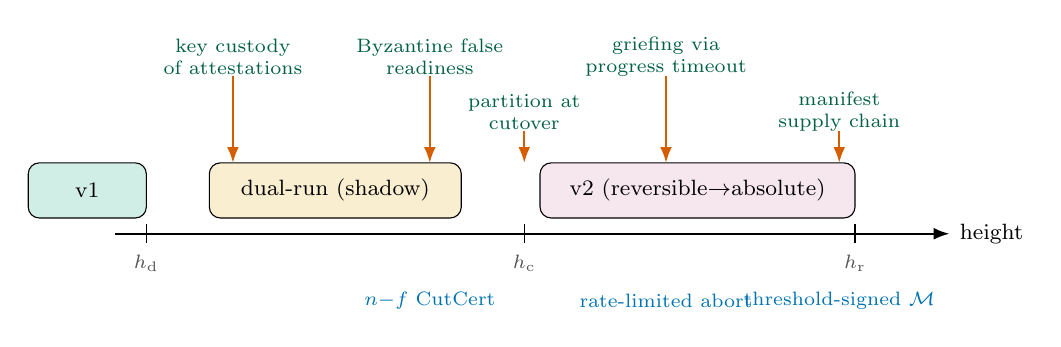
\begin{tikzpicture}[
  font=\footnotesize,
  phase/.style={draw, rounded corners, minimum height=7mm, align=center, fill=#1},
  atk/.style={-{Latex[length=2mm]}, thick, color=cbRed},
  mit/.style={font=\scriptsize, color=cbGreen!60!black, align=center},
  lab/.style={font=\scriptsize, color=cbGray}
]
% timeline axis
\draw[thick,-{Latex[length=2mm]}] (0,0) -- (10.6,0) node[right]{height};
\foreach \x/\t in {0.4/$h_{\mathrm{d}}$, 5.2/$h_{\mathrm{c}}$, 9.4/$h_{\mathrm{r}}$}{
  \draw (\x,0.12) -- (\x,-0.12); \node[lab, below] at (\x,-0.15){\t};
}
% phase bands
\node[phase=cbGreen!18, minimum width=1.5cm] at (-0.35,0.55) {v1};
\node[phase=cbOrange!18, minimum width=3.2cm] at (2.8,0.55) {dual-run (shadow)};
\node[phase=cbPurple!18, minimum width=4.0cm] at (7.4,0.55) {v2 (reversible$\to$absolute)};
% attacks above
\node[mit] at (1.5,2.25) {key custody\\of attestations};
\draw[atk] (1.5,2.0) -- (1.5,0.9);
\node[mit] at (4.0,2.25) {Byzantine false\\readiness};
\draw[atk] (4.0,2.0) -- (4.0,0.9);
\node[mit] at (5.2,1.55) {partition at\\cutover};
\draw[atk] (5.2,1.3) -- (5.2,0.9);
\node[mit] at (7.0,2.25) {griefing via\\progress timeout};
\draw[atk] (7.0,2.0) -- (7.0,0.9);
\node[mit] at (9.2,1.55) {manifest\\supply chain};
\draw[atk] (9.2,1.3) -- (9.2,0.9);
% mitigations below
\node[mit, text=cbBlue] at (4.0,-0.85) {$n{-}f$ CutCert};
\node[mit, text=cbBlue] at (7.0,-0.85) {rate-limited abort};
\node[mit, text=cbBlue] at (9.2,-0.85) {threshold-signed $\mathcal{M}$};
\end{tikzpicture}}
\caption{Attack surfaces across the migration timeline and their mitigations. Cutover safety
rests on the $n-f$ CutCert (quorum intersection), reversibility on the threshold-signed
manifest, and liveness on a rate-limited abort path.}
\label{fig:threat}
\end{figure}

\emph{Partition at cutover.} A partition straddling $h_{\mathrm{c}}$ is the canonical way a
flag-day fork arises: two sides each proceed on their own chain. SAGE neutralizes this because
cutover requires an $n-f$ CutCert, and by quorum intersection (Lemma~\ref{lem:qi}) at most one
partition side can assemble it; the other side keeps the legacy chain and adopts the CutCert
after the partition heals. \emph{Byzantine false readiness.} A Byzantine validator may sign a
readiness attestation for a height at which its local shadow check failed. Because a CutCert
needs $n-f$ signatures and $f<n/3$, every CutCert contains at least $f+1$ correct signers, so
the certified root equals the legacy-finalized root (Theorem~\ref{th:safety}).
\emph{Griefing via the progress timeout.} A Byzantine coalition can stall $\mathcal{C}_2$ to
trip the progress timeout $\tau$ and force a rollback, then repeat. SAGE bounds this by
rate-limiting forced rollbacks to a constant per epoch and by requiring an $n-f$ AbortCert for
a quorum-triggered abort, so $f$ validators cannot by themselves trigger the quorum path; the
timeout path is bounded in Section~\ref{sec:analysis}. \emph{Manifest supply chain.} A
malicious migration tool could emit a state that is internally consistent but wrong. The
manifest binds the tool hash and is threshold-signed by validators that independently
recompute the boundary root, so a single compromised tool cannot pass verification; we treat
collusion of $f+1$ key holders as out of scope, consistent with the BFT bound.

\begin{table}[t]
\centering
\caption{Abort triggers, the adversary that can invoke each, and the resulting guarantee.}
\label{tab:abort}
\setlength{\tabcolsep}{4pt}
\renewcommand{\arraystretch}{1.2}
\footnotesize
\begin{tabular}{p{0.27\columnwidth}p{0.30\columnwidth}p{0.30\columnwidth}}
\toprule
Trigger & Who can invoke & Guarantee \\
\midrule
Progress timeout $\tau$ & any (incl.\ $f$ Byzantine stalling) & rate-limited; rollback converges (Thm.~\ref{th:rollback}) \\
Quorum abort ($n{-}f$) & needs $\ge f{+}1$ correct & cannot be forced by $f$ Byzantine \\
Manifest mismatch & detected locally by any correct node & tamper-evident (Thm.~\ref{th:unforge}) \\
\bottomrule
\end{tabular}
\end{table}

% ===================== PROTOCOL =====================
\section{The SAGE Protocol}
\label{sec:protocol}

SAGE (Shadow-Anchored Graceful Evolution) realizes a heterogeneous engine migration through
four mechanisms: a single-finalizer dual-run invariant, a quorum-certified cutover decision,
a threshold-signed migration manifest, and a deadline-bounded rollback under a two-tier
finality model. Fig.~\ref{fig:arch} shows the data path, Fig.~\ref{fig:seq} the temporal
message flow, and Fig.~\ref{fig:schedule} the controller as a labeled transition system.

\begin{figure*}[t]
\centering
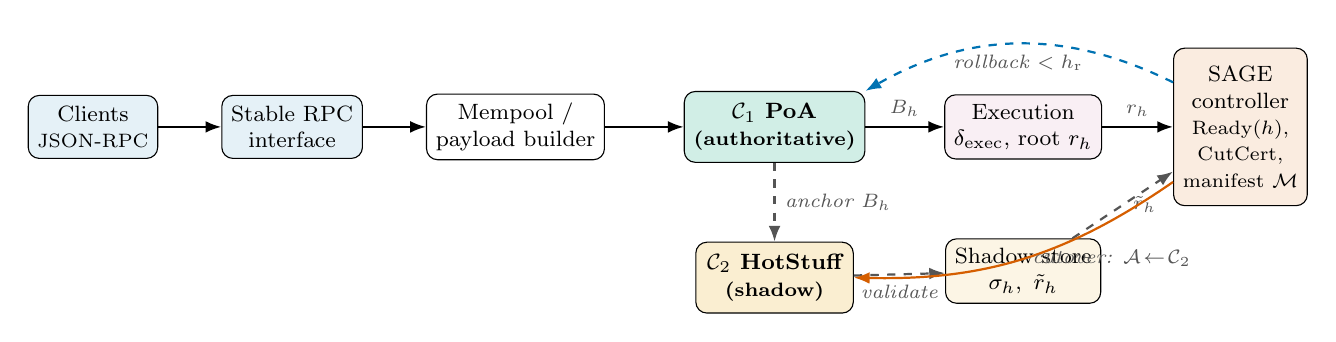
\begin{tikzpicture}[
  node distance=6mm,
  box/.style={draw, rounded corners, align=center, minimum height=8mm, font=\footnotesize, fill=white},
  eng/.style={draw, rounded corners, align=center, minimum height=9mm, minimum width=20mm, font=\footnotesize\bfseries},
  lab/.style={font=\scriptsize\itshape, text=cbGray},
  arr/.style={-{Latex[length=2mm]}, thick},
  darr/.style={-{Latex[length=2mm]}, thick, dashed, color=cbGray}
]
\node[box, fill=cbBlue!10] (client) {Clients\\\scriptsize JSON-RPC};
\node[box, right=8mm of client, fill=cbBlue!10] (rpc) {Stable RPC\\interface};
\node[box, right=8mm of rpc] (pool) {Mempool /\\payload builder};
\node[eng, right=10mm of pool, fill=cbGreen!18] (c1) {$\mathcal{C}_1$ PoA\\\scriptsize (authoritative)};
\node[eng, below=10mm of c1, fill=cbOrange!18] (c2) {$\mathcal{C}_2$ HotStuff\\\scriptsize (shadow)};
\node[box, right=10mm of c1, fill=cbPurple!12] (exec) {Execution\\$\delta_{\mathrm{exec}}$, root $r_h$};
\node[box, below=10mm of exec, fill=cbOrange!10] (shadow) {Shadow store\\$\sigma_h,\ \tilde r_h$};
\node[box, right=9mm of exec, fill=cbRed!12, minimum height=20mm] (ctrl) {SAGE\\controller\\\scriptsize Ready$(h)$,\\\scriptsize CutCert,\\\scriptsize manifest $\mathcal{M}$};
\draw[arr] (client) -- (rpc);
\draw[arr] (rpc) -- (pool);
\draw[arr] (pool) -- (c1);
\draw[arr] (c1) -- node[lab, above]{$B_h$} (exec);
\draw[arr] (exec) -- node[lab, above]{$r_h$} (ctrl);
\draw[darr] (c1) -- node[lab, right]{anchor $B_h$} (c2);
\draw[darr] (c2) -- node[lab, below]{validate} (shadow);
\draw[darr] (shadow) -- node[lab, right]{$\tilde r_h$} (ctrl);
\draw[arr, color=cbRed] (ctrl) to[bend left=18] node[lab, right]{cutover: $\mathcal{A}\!\leftarrow\!\mathcal{C}_2$} (c2.east);
\draw[darr, color=cbBlue] (ctrl) to[bend right=28] node[lab, below]{rollback $<h_{\mathrm{r}}$} (c1.north east);
\end{tikzpicture}
\caption{SAGE data path during dual-run. The legacy engine $\mathcal{C}_1$ is the sole
finalizer and feeds each canonical block $B_h$ to the target engine $\mathcal{C}_2$, which
validates it in shadow mode and records a verdict $\sigma_h$ and a recomputed root
$\tilde r_h$. The controller evaluates the readiness predicate, assembles the CutCert, commits
the threshold-signed manifest at cutover, and can transfer authority to $\mathcal{C}_2$ or
roll back to $\mathcal{C}_1$ before the deadline. The client RPC interface is invariant
throughout.}
\label{fig:arch}
\end{figure*}

\begin{figure}[t]
\centering
\resizebox{\columnwidth}{!}{%
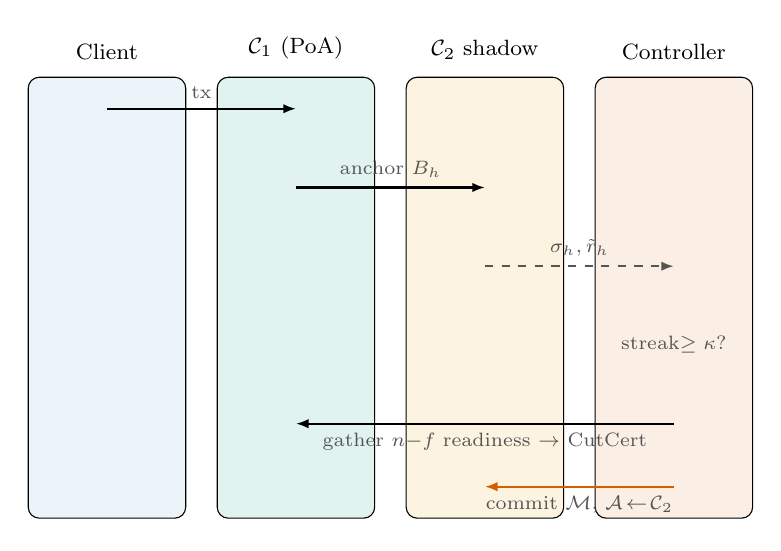
\begin{tikzpicture}[font=\footnotesize,
  lane/.style={draw, rounded corners, fill=#1, minimum width=2.0cm, minimum height=5.6cm, align=center},
  msg/.style={-{Latex[length=1.6mm]}, thick},
  dmsg/.style={-{Latex[length=1.6mm]}, thick, dashed, color=cbGray},
  note/.style={font=\scriptsize, color=cbGray}
]
% lanes
\node[lane=cbBlue!8]  (cl) at (0,0)   {}; \node[above=1mm of cl]{Client};
\node[lane=cbGreen!12](v1) at (2.4,0) {}; \node[above=1mm of v1]{$\mathcal{C}_1$ (PoA)};
\node[lane=cbOrange!12](v2) at (4.8,0){}; \node[above=1mm of v2]{$\mathcal{C}_2$ shadow};
\node[lane=cbRed!10]  (ct) at (7.2,0) {}; \node[above=1mm of ct]{Controller};
% lifelines y positions from top 2.6 down to -2.6
\def\yA{2.4} \def\yB{1.4} \def\yC{0.4} \def\yD{-0.6} \def\yE{-1.6} \def\yF{-2.4}
% tx flow
\draw[msg] (cl.north |- 0,\yA) ++(0,0) -- (v1.north |- 0,\yA);
\node[note, above] at (1.2,\yA){tx};
\draw[msg] (2.4,\yB) -- (4.8,\yB); \node[note,above] at (3.6,\yB){anchor $B_h$};
\draw[dmsg] (4.8,\yC) -- (7.2,\yC); \node[note,above] at (6.0,\yC){$\sigma_h,\tilde r_h$};
\node[note] at (7.2,\yD){streak$\ge\kappa$?};
\draw[msg] (7.2,\yE) -- (2.4,\yE); \node[note,below] at (4.8,\yE){gather $n{-}f$ readiness $\to$ CutCert};
\draw[msg, color=cbRed] (7.2,\yF) -- (4.8,\yF); \node[note,below] at (6.0,\yF){commit $\mathcal{M}$, $\mathcal{A}\!\leftarrow\!\mathcal{C}_2$};
\end{tikzpicture}}
\caption{Temporal message flow for one dual-run cycle and the cutover. The client sees an
unchanged interface; the legacy engine finalizes and anchors each block to the shadow target;
the controller accumulates shadow verdicts, and once the stability streak is reached it
gathers an $n-f$ readiness quorum into a CutCert, commits the threshold-signed manifest, and
transfers authority.}
\label{fig:seq}
\end{figure}

\begin{figure}[t]
\centering
\resizebox{\columnwidth}{!}{%
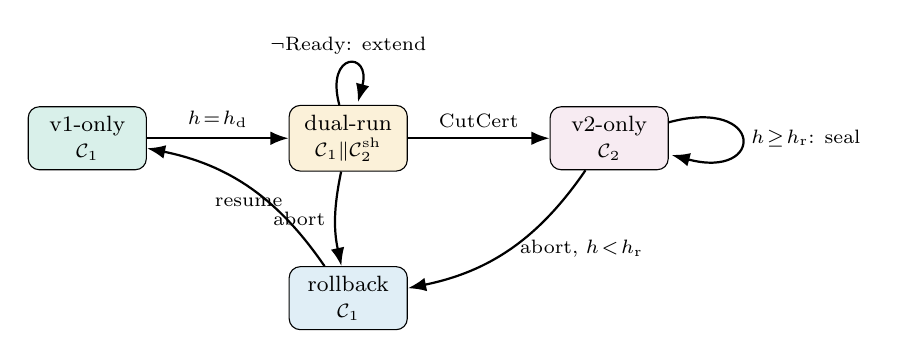
\begin{tikzpicture}[
  >=Latex, node distance=18mm,
  state/.style={draw, rounded corners, minimum width=15mm, minimum height=8mm, align=center, font=\footnotesize, fill=cbBlue!8},
  every edge/.style={draw, ->, thick},
  lab/.style={font=\scriptsize}
]
\node[state, fill=cbGreen!15] (v1) {v1-only\\\scriptsize $\mathcal{C}_1$};
\node[state, right=of v1, fill=cbOrange!15] (dual) {dual-run\\\scriptsize $\mathcal{C}_1\|\mathcal{C}_2^{\mathrm{sh}}$};
\node[state, right=of dual, fill=cbPurple!15] (v2) {v2-only\\\scriptsize $\mathcal{C}_2$};
\node[state, below=12mm of dual, fill=cbBlue!12] (rb) {rollback\\\scriptsize $\mathcal{C}_1$};
\path (v1) edge node[lab, above]{$h\!=\!h_{\mathrm{d}}$} (dual);
\path (dual) edge node[lab, above]{CutCert} (v2);
\path (dual) edge[loop above] node[lab]{$\neg$Ready: extend} (dual);
\path (dual) edge[bend right=12] node[lab, left]{abort} (rb);
\path (v2) edge[bend left=22] node[lab, right]{abort, $h\!<\!h_{\mathrm{r}}$} (rb);
\path (rb) edge[bend right=22] node[lab, below]{resume} (v1);
\path (v2) edge[loop right] node[lab, right]{$h\!\ge\!h_{\mathrm{r}}$: seal} (v2);
\end{tikzpicture}}
\caption{SAGE as a labeled transition system with explicit precedence: abort dominates
cutover at the same height, and dual-run self-loops (extends) while the readiness predicate is
false, so the system is never undefined when stability is not reached by the scheduled height.}
\label{fig:schedule}
\end{figure}

\subsection{Migration Schedule as a Transition System}
A migration is governed by three heights $h_{\mathrm{d}} < h_{\mathrm{c}} \le h_{\mathrm{r}}$
fixed in platform state $P$ and amendable only through the legacy engine before
$h_{\mathrm{d}}$. Rather than a piecewise height function with overlapping cases, we define the
active engine by the labeled transition system of Fig.~\ref{fig:schedule}, with states
$\{\textsc{v1},\textsc{dual},\textsc{v2},\textsc{rollback},\textsc{sealed}\}$ and a fixed
precedence: at any height an enabled abort transition dominates an enabled cutover transition,
and the dual-run state self-loops while the readiness predicate is false. The authoritative
engine $\mathcal{A}(h)$ is $\mathcal{C}_1$ in states \textsc{v1}, \textsc{dual}, and
\textsc{rollback}, and $\mathcal{C}_2$ in \textsc{v2} and \textsc{sealed}. This removes the
ambiguity of an unconditional height-indexed switch: the system has a defined successor in
every state, including the case where stability is not reached by $h_{\mathrm{c}}$, in which
case dual-run is extended.

\subsection{Single-Finalizer Dual-Run}
The central invariant is that at every height exactly one engine finalizes. During
$[h_{\mathrm{d}}, h_{\mathrm{c}})$ the legacy engine $\mathcal{C}_1$ is the sole authority: it
orders and finalizes $B_h$ exactly as before $h_{\mathrm{d}}$. The target engine
$\mathcal{C}_2$ does not propose; it consumes the already-finalized $B_h$, runs its own
validation routine, and records a verdict $\sigma_h$ and the root $\tilde r_h$ it computes for
the same transactions.

\begin{definition}[Shadow mode]
\label{def:shadow}
An engine runs in shadow mode at height $h$ if, for the canonical block $B_h$ finalized by the
authoritative engine, each correct validator runs the shadow engine's validation routine on
$B_h$, records $\sigma_h \in \{\mathsf{valid},\mathsf{invalid}\}$ and $\tilde r_h$ (with
$\tilde r_h=\bot$ if validation rejects), and does not propose or finalize any block. Shadow
validation is a side-effect-free function of $(B_h,S_{h-1})$ and never blocks the finalization
path.
\end{definition}

\subsection{Quorum-Certified Cutover Decision}
Cutover is not a local choice; it is a single agreed decision carried by a certificate.

\begin{definition}[Readiness attestation and CutCert]
\label{def:cutcert}
A correct validator $i$ emits a readiness attestation $\mathsf{att}_i(h) = \mathrm{Sign}_i
\langle \textsc{ready}, \mathrm{cid}, e, h, r_h\rangle$ only if its last $\kappa$ shadow
verdicts were $\mathsf{valid}$ with $\tilde r_j = r_j$ for $j\in[h-\kappa+1,h]$, where
$\mathrm{cid}$ is the chain identifier and $e$ the migration epoch. A CutCert for height
$h_{\mathrm{c}}$ is a set of $n-f$ attestations on the same $\langle \mathrm{cid},e,h_{\mathrm{c}}-1,r\rangle$,
aggregated into a threshold signature.
\end{definition}

\subsection{Threshold-Signed Migration Manifest}
The boundary is bound by a manifest that is cryptographically signed and replay-bound, not a
bare equality check:
\begin{equation}
\mathcal{M} = \big\langle \mathrm{cid}, e, h_{\mathrm{c}}, \mathsf{H}(B_{h_{\mathrm{c}}-1}),
r_{h_{\mathrm{c}}-1}, g_1, g_2, \mathsf{H}_{\mathrm{tool}}, \pi \big\rangle,
\end{equation}
where $g_1,g_2$ are the engine generation identifiers, $\mathsf{H}_{\mathrm{tool}}$ binds the
migration tooling, and $\pi$ is the threshold signature of the CutCert over the tuple. A
correct validator accepts cutover only if (i) $\pi$ verifies as an $n-f$ threshold signature,
(ii) the carried root equals the validator's locally recomputed
$\mathrm{root}(S_{h_{\mathrm{c}}-1})$, and (iii) $\mathcal{M}$ is carried in a
$\mathcal{C}_1$-finalized header. The chain identifier and epoch make a manifest from one
migration or chain non-replayable on another.

\subsection{Two-Tier Finality and Bounded Rollback}
To reconcile reversibility with client semantics we adopt two finality tiers. A block is
\emph{absolutely final} if $h < h_{\mathrm{c}}$ (legacy-finalized) or $h \ge h_{\mathrm{r}}$
(sealed target). A block in the reversible window $[h_{\mathrm{c}}, h_{\mathrm{r}})$ is
\emph{provisionally final}: clients are told through an advisory finality flag that it may be
reverted until $h_{\mathrm{r}}$. The abort condition $\textsc{AbortCondition}(h)$ fires when
the target produces no finalized block within the progress timeout $\tau$, when an $n-f$
AbortCert is formed, or when manifest verification fails. On abort before $h_{\mathrm{r}}$ the
controller discards the provisional suffix, resets $\mathcal{A}$ to $\mathcal{C}_1$ at
$S_{h_{\mathrm{c}}-1}$, and resumes legacy finalization; transactions in the discarded suffix
are deterministically replayed onto $\mathcal{C}_1$. After $h_{\mathrm{r}}$ the target is
sealed and rollback is disabled. The advisory flag is the only client-visible change, so a
client that honors provisional finality observes a monotone, uninterrupted chain; this is the
precise sense in which SAGE preserves the client interface.

\begin{algorithm}[t]
\caption{SAGE per-height controller at a correct validator}
\label{alg:sage}
\begin{algorithmic}[1]
\Require schedule $(h_{\mathrm{d}}, h_{\mathrm{c}}, h_{\mathrm{r}})$, threshold $\kappa$, timeout $\tau$
\State $\mathit{state} \gets \textsc{v1}$;\ \ $\mathit{streak} \gets 0$
\For{each finalized canonical block $B_h$ with root $r_h$}
  \If{$\mathit{state}=\textsc{v1}$ \textbf{and} $h \ge h_{\mathrm{d}}$}\ $\mathit{state}\gets\textsc{dual}$\ \EndIf
  \If{\Call{AbortCondition}{$h,\tau$} \textbf{and} $h < h_{\mathrm{r}}$}
     \State $\mathcal{A}\gets\mathcal{C}_1$ at $S_{h_{\mathrm{c}}-1}$;\ replay suffix;\ $\mathit{state}\gets\textsc{rollback}$;\ \textbf{continue}
  \EndIf
  \If{$\mathit{state}=\textsc{dual}$}
     \State $(\sigma_h,\tilde r_h)\gets\mathcal{C}_2.\textsc{ShadowValidate}(B_h)$
     \State \textbf{if} $\sigma_h{=}\mathsf{valid}\wedge\tilde r_h{=}r_h$ \textbf{then} $\mathit{streak}{+}{+}$ \textbf{else} $\mathit{streak}\gets 0$
     \If{$\mathit{streak}\ge\kappa$ \textbf{and} $h{+}1\ge h_{\mathrm{c}}$}
        \State broadcast $\mathsf{att}_i(h)$;\ collect $n{-}f$ into $\mathrm{CutCert}$
        \If{$\mathrm{CutCert}$ formed}
           \State $\mathcal{M}\gets\mathrm{sign}(\mathrm{cid},e,h{+}1,\mathsf{H}(B_h),r_h,\ldots)$
           \State commit $\mathcal{M}$;\ $C\gets\mathcal{C}_2.\mathsf{Init}(r_h,h{+}1)$
           \State $\mathcal{A}\gets\mathcal{C}_2$;\ $\mathit{state}\gets\textsc{v2}$
        \EndIf
     \EndIf
  \EndIf
  \If{$h\ge h_{\mathrm{r}}$}\ seal target;\ $\mathit{state}\gets\textsc{sealed}$ \EndIf
\EndFor
\end{algorithmic}
\end{algorithm}

\subsection{Design Rationale: Why Each Mechanism Is Necessary}
Each of SAGE's four mechanisms removes a specific failure that the others do not cover, and the
evaluation in Section~\ref{sec:eval} treats these failures as falsifiable invariant checks.
The \emph{single-finalizer dual-run} is what prevents two engines from ever both finalizing;
without it, running two engines in parallel is a latent fork waiting for a partition. The RQ2
exposure metric (Section~\ref{sec:eval}) makes this concrete: under a cutover-straddling
partition with a balanced split, hard fork and blind cutover are exposed to a disjoint-quorum
fork window in $100\%$ of trials while SAGE is exposed in $0\%$. The
\emph{quorum-certified cutover} is what makes the switch a single agreed decision; without it, a
blind schedule lets each partition side switch independently, which is exactly the exposure the
metric records. The \emph{threshold-signed manifest} is what makes the boundary
auditable and the rollback verifiable; a bare equality check, as a naive design might use, binds
a value to itself and is forgeable by any proposer, so the unforgeability and replay-resistance
theorems would not hold. The \emph{two-tier finality} is what reconciles reversibility with the
client contract; without an explicit provisional tier, a rollback would revert blocks a client
was told were final, which is a finality reversion and a client-visible safety violation. The
design is therefore minimal in the sense that dropping any one mechanism reintroduces a concrete
failure that the evaluation can produce.

% ===================== ANALYSIS =====================
\section{Theoretical Analysis}
\label{sec:analysis}

We prove decision uniqueness, cross-boundary safety, quantified liveness, migration
termination, rollback correctness, manifest security, the detection bound, and complexity. We
first state the assumptions and the vocabulary the theorems quantify over.

\begin{assumption}[Engine correctness]
\label{as:engines}
Each engine conforms to Definition~\ref{def:engine}. $\mathcal{C}_1$ provides safety under its
authority quorum $\mathsf{Q}_1$, and $\mathcal{C}_2$ provides safety always and liveness after
GST under $\mathsf{Q}_2=2f_2+1$ with $n\ge 3f_2+1$.
\end{assumption}

\begin{assumption}[Deterministic execution]
\label{as:exec}
$\delta_{\mathrm{exec}}$ is deterministic on well-formed blocks, so two correct validators
that apply the same block sequence from the same initial state compute identical roots.
\end{assumption}

\begin{assumption}[Cryptography]
\label{as:crypto}
$\mathrm{root}(\cdot)$ and $\mathsf{H}$ are collision resistant and the threshold signature is
EUF-CMA secure; the adversary controls at most $f<n/3$ keys.
\end{assumption}

\begin{definition}[Commit and convergence]
\label{def:commit}
$\mathrm{committed}_i(h,B)$ holds if correct validator $i$ has a finalization certificate for
block $B$ at height $h$. Two correct validators \emph{conflict} at $h$ if they commit distinct
blocks. The system \emph{converges} if the committed prefixes of all correct validators are
eventually identical.
\end{definition}

\begin{lemma}[Quorum intersection]
\label{lem:qi}
With $n\ge 3f+1$, any two $(n-f)$-quorums intersect in at least $n-2f\ge f+1$ validators, hence
in at least one correct validator.
\end{lemma}
\begin{proof}
Two sets of size $n-f$ in a universe of size $n$ intersect in at least $2(n-f)-n = n-2f$
elements. With $n\ge 3f+1$, $n-2f\ge f+1$. Since at most $f$ validators are Byzantine, an
intersection of size $\ge f+1$ contains at least one correct validator.
\end{proof}

\begin{theorem}[Decision uniqueness]
\label{th:unique}
For a fixed migration epoch $e$, at most one CutCert can be formed, and it fixes a unique
cutover height $h_{\mathrm{c}}$ and boundary root $r$. Symmetrically at most one of a CutCert
or an $(n-f)$ AbortCert is valid at the same height. Consequently every correct validator that
acts on a valid certificate takes the same action.
\end{theorem}
\begin{proof}
A CutCert requires $n-f$ attestations on the same $\langle\mathrm{cid},e,h_{\mathrm{c}}-1,r\rangle$
(Definition~\ref{def:cutcert}). Suppose two CutCerts existed for epoch $e$ with distinct
$(h_{\mathrm{c}},r)$ values. Each is signed by an $(n-f)$-quorum; by Lemma~\ref{lem:qi} the two
quorums share a correct validator. A correct validator signs at most one readiness attestation
per epoch (it tracks the epoch in $P$), so it cannot have signed two distinct tuples,
contradiction. The same intersection argument applies to a CutCert and an AbortCert: a shared
correct validator would have to have signed both a readiness and an abort message for epoch
$e$, which the controller forbids. Authenticity of the certificate follows from EUF-CMA
security (Assumption~\ref{as:crypto}), so a Byzantine coalition of size $f$ cannot fabricate
either certificate. Hence at most one decision exists and all correct validators act on it
identically.
\end{proof}

\begin{lemma}[Single finalizer during dual-run]
\label{lem:single}
For every height $h\in[h_{\mathrm{d}},h_{\mathrm{c}})$ only $\mathcal{C}_1$ finalizes, and at
most one block is finalized at $h$.
\end{lemma}
\begin{proof}
In state \textsc{dual} the authoritative engine is $\mathcal{C}_1$. By
Definition~\ref{def:shadow} the shadow engine neither proposes nor finalizes; it only validates
the block already finalized by $\mathcal{C}_1$. Finalization at $h$ is therefore governed solely
by $\mathcal{C}_1$, which finalizes at most one block per height (Assumption~\ref{as:engines}).
\end{proof}

\begin{theorem}[Cross-boundary safety]
\label{th:safety}
No two correct validators conflict at any height, including the boundary $h_{\mathrm{c}}$.
\end{theorem}
\begin{proof}
We prove the inductive invariant $I$: ``at every height $h$ exactly one block holds a
finalization certificate, and every correct validator's committed prefix is a prefix of a
single canonical chain from genesis.'' \emph{Base.} Before $h_{\mathrm{d}}$ only $\mathcal{C}_1$
is active and $I$ holds by Assumption~\ref{as:engines}. \emph{Induction, dual-run.} For
$h\in[h_{\mathrm{d}},h_{\mathrm{c}})$, Lemma~\ref{lem:single} gives a unique finalized block, so
$I$ is preserved. \emph{Induction, boundary.} Cutover occurs only with a valid CutCert
(Theorem~\ref{th:unique}), which contains $n-f\ge 2f+1$ attestations, hence at least $f+1$
correct ones (Lemma~\ref{lem:qi}). Each correct attestor signed $\langle\cdot,h_{\mathrm{c}}-1,r\rangle$
only after locally verifying $\tilde r_{h_{\mathrm{c}}-1}=r_{h_{\mathrm{c}}-1}$, and by
Assumption~\ref{as:exec} all correct validators compute the same root for the agreed prefix.
The manifest's acceptance rule (ii) forces every correct validator to recompute and match this
root, and $\mathcal{C}_2.\mathsf{Init}$ (Definition~\ref{def:bootstrap}) seeds the target from
exactly $r_{h_{\mathrm{c}}-1}$. Thus $\mathcal{C}_2$ extends the unique legacy prefix, and any
block it finalizes at $h_{\mathrm{c}}$ continues the single canonical chain, preserving $I$.
\emph{Induction, target.} For $h>h_{\mathrm{c}}$ only $\mathcal{C}_2$ is authoritative and its
standalone safety preserves $I$. Since $I$ implies no conflict at any height, the claim
follows.
\end{proof}

\begin{theorem}[Quantified zero-halt liveness]
\label{th:liveness}
After GST with $n\ge 3f+1$, inter-commit time is at most $T_{\mathrm{dual}}$ during dual-run
and at most $T_{\mathrm{bdy}} = T_{\mathrm{init}} + 2\Delta$ across the handoff, where
$T_{\mathrm{init}}$ is the target engine's first-view cost; block production never halts during
migration.
\end{theorem}
\begin{proof}
During dual-run the authoritative engine is $\mathcal{C}_1$, which finalizes within its normal
round time $T_{\mathrm{dual}}$; shadow validation is a non-blocking side-effect-free function
(Definition~\ref{def:shadow}) executed after finalization, so it cannot extend the critical
path, hence inter-commit time is $T_{\mathrm{dual}}$. The cutover step gathers an $n-f$ CutCert;
after GST a correct quorum responds within $\Delta$, and certificate verification is local. The
target then runs its first view: leader election and pacemaker initialization complete within
$T_{\mathrm{init}}$, and the first quorum certificate forms within one additional round, bounded
by $2\Delta$ after GST. Thus the handoff adds at most $T_{\mathrm{bdy}}=T_{\mathrm{init}}+2\Delta$
between the last $\mathcal{C}_1$ commit and the first $\mathcal{C}_2$ commit. No state introduces
a stop step, so inter-commit time is bounded throughout and production never halts.
\end{proof}

\begin{corollary}[No observable service interruption]
\label{cor:nohalt}
Under the conditions of Theorem~\ref{th:liveness}, a client that submits transactions throughout
the migration observes a finalization stream whose maximum inter-commit gap is
$\max(T_{\mathrm{dual}}, T_{\mathrm{bdy}})$, independent of the migration itself.
\end{corollary}
\begin{proof}
Immediate from Theorem~\ref{th:liveness} and Proposition~\ref{prop:bdy}: every regime has a live
finalizer and the handoff gap is bounded by $T_{\mathrm{bdy}}$, so the client-visible stream
never stalls beyond the larger of the two bounds.
\end{proof}

\begin{theorem}[Migration termination]
\label{th:termination}
After GST with $n\ge 3f+1$ and no shadow-invalid blocks, the readiness streak reaches $\kappa$
within $\kappa$ heights, an $n-f$ CutCert forms within $\Delta$, and cutover completes; if a
partition prevents an $n-f$ quorum, cutover completes within $\Delta$ after the partition
heals.
\end{theorem}
\begin{proof}
With no shadow-invalid blocks the streak increments each height and reaches $\kappa$ after
$\kappa$ heights (Algorithm~\ref{alg:sage}, line~9). After GST a correct $(n-f)$-quorum exchanges
readiness attestations within $\Delta$, forming a CutCert (Definition~\ref{def:cutcert}); by
Theorem~\ref{th:unique} it is unique, and cutover follows. If a partition leaves no side with
$n-f$ correct validators, no CutCert forms and the system self-loops in \textsc{dual}
(Fig.~\ref{fig:schedule}); once the partition heals, the full correct set, of size $\ge n-f$,
forms a CutCert within $\Delta$. Hence migration terminates.
\end{proof}

\begin{theorem}[Rollback correctness]
\label{th:rollback}
If an abort fires at height $h_a<h_{\mathrm{r}}$, every correct validator converges to the
legacy-finalized state $S_{h_{\mathrm{c}}-1}$ with no conflict on absolutely final blocks, and
any tampering with the resumed state is detected.
\end{theorem}
\begin{proof}
Blocks in $[h_{\mathrm{c}},h_a]$ are only provisionally final by the two-tier model, so no
absolutely final block is reverted and the client contract on absolute finality is preserved.
The controller retains the $\mathcal{C}_1$ finalization certificate for $S_{h_{\mathrm{c}}-1}$
until $h_{\mathrm{r}}$. On abort it discards the provisional suffix and resets authority to
$\mathcal{C}_1$ at $S_{h_{\mathrm{c}}-1}$. By Theorem~\ref{th:safety} the suffix extended the
unique legacy prefix, so removing it orphans no independently legacy-finalized block.
Convergence to $S_{h_{\mathrm{c}}-1}$ follows from the retained certificate and
Assumption~\ref{as:exec}, and suffix transactions are replayed deterministically onto
$\mathcal{C}_1$. If an adversary attempts to resume from $S'\ne S_{h_{\mathrm{c}}-1}$, its root
$r'\ne r_{h_{\mathrm{c}}-1}$ fails manifest acceptance rule (ii) at every correct validator, so
the resume is rejected. By Theorem~\ref{th:unique} the abort decision is unique, so all correct
validators roll back identically. The progress-timeout path is rate-limited to a constant per
epoch, so $f$ Byzantine validators that stall $\mathcal{C}_2$ cannot force unbounded rollbacks.
\end{proof}

\begin{theorem}[Manifest unforgeability]
\label{th:unforge}
Under Assumptions~\ref{as:crypto}, an adversary controlling $\le f$ keys cannot produce an
accepted manifest whose committed boundary state differs from the unique legacy-finalized
$S_{h_{\mathrm{c}}-1}$, except with negligible probability.
\end{theorem}
\begin{proof}
An accepted manifest carries a threshold signature $\pi$ that verifies as $n-f$ signatures
(rule (i)). Suppose an adversary outputs an accepted $\mathcal{M}$ with root
$r'\ne r_{h_{\mathrm{c}}-1}$. Either (a) $\pi$ aggregates a signature from a correct validator on
$r'$, which a correct validator never produces because it signs only its locally recomputed root
(Definition~\ref{def:cutcert}); by Lemma~\ref{lem:qi} an $n-f$ set contains $\ge f+1$ correct
validators, so at least one correct signature on $r'$ is required, contradiction; or (b) the
adversary forged a correct validator's signature, breaking EUF-CMA, which occurs with negligible
probability; or (c) $r'$ collides with $r_{h_{\mathrm{c}}-1}$ under $\mathrm{root}(\cdot)$, which
contradicts collision resistance. Hence acceptance of a wrong-state manifest is negligible.
\end{proof}

\begin{theorem}[Replay resistance]
\label{th:replay}
A manifest valid for $(\mathrm{cid},e)$ does not verify for any $(\mathrm{cid}',e')\ne
(\mathrm{cid},e)$.
\end{theorem}
\begin{proof}
The signed tuple includes $\mathrm{cid}$ and $e$, and attestations are over the same fields
(Definition~\ref{def:cutcert}). Verification recomputes the signed message with the local
$(\mathrm{cid}',e')$; a single differing field changes the message, so $\pi$ fails to verify by
EUF-CMA correctness unless the adversary forges a signature on the new message, which is
negligible.
\end{proof}

\begin{theorem}[Detection probability]
\label{th:detection}
Let a latent divergence be present with probability $p_{\mathrm{div}}$ and detected per shadow
block with probability $q$. The probability of an unsafe cutover under threshold $\kappa$ is
$\Pr[\mathrm{unsafe}] = p_{\mathrm{div}}(1-q)^{\kappa}$, which decreases geometrically in
$\kappa$.
\end{theorem}
\begin{proof}
A cutover is unsafe only if a divergence is present and escapes detection across all $\kappa$
blocks of the stability window. Detections are independent per block with miss probability
$1-q$, so the divergence escapes the window with probability $(1-q)^{\kappa}$. Multiplying by the
presence probability gives $p_{\mathrm{div}}(1-q)^{\kappa}$. For $q>0$ this tends to $0$ as
$\kappa\to\infty$.
\end{proof}

\begin{theorem}[Message and round complexity]
\label{th:complexity}
Dual-run adds zero wire messages per block. Cutover costs $O(n)$ messages per collector (or
$O(n^2)$ all-to-all) and $O(1)$ extra rounds; abort costs the same. Steady-state per-engine
complexity is unchanged.
\end{theorem}
\begin{proof}
Shadow validation is local (Definition~\ref{def:shadow}), adding no messages. Forming a CutCert
gathers $n-f=O(n)$ attestations, $O(n)$ at a designated collector or $O(n^2)$ broadcast, in one
round; threshold aggregation and verification are $O(n)$ work but $O(1)$ rounds. The AbortCert is
symmetric. Outside the one-time decision, each engine runs unchanged, so steady-state complexity
is preserved.
\end{proof}

\begin{proposition}[Boundary latency]
\label{prop:bdy}
After GST, the gap between the last legacy commit and the first target commit is at most
$T_{\mathrm{bdy}} = \Delta_{\mathrm{cert}} + T_{\mathrm{init}} + 2\Delta$, where
$\Delta_{\mathrm{cert}}$ is the one-round CutCert gather, $T_{\mathrm{init}}$ is the target
first-view setup, and $2\Delta$ bounds the first target quorum certificate.
\end{proposition}
\begin{proof}
The CutCert gathers $n-f$ attestations in one post-GST round, so it forms within
$\Delta_{\mathrm{cert}}\le\Delta$ plus $O(n)$ local verification. The target then runs
$\mathsf{Init}$ in $T_{\mathrm{init}}$ and its first view completes a quorum certificate within
two message delays after GST. Summing the three terms gives the bound; none is unbounded after
GST, so the handoff cannot stall.
\end{proof}

\subsection{Overhead Analysis}
Before $h_{\mathrm{d}}$ and after $h_{\mathrm{c}}$ SAGE adds no work to the finalization path.
During dual-run each correct validator performs one shadow validation per block, costing
$O(|B_h|)$ re-execution plus an $O(1)$ root comparison; since this is off the critical path the
measured throughput overhead is small and roughly constant in $n$ (Section~\ref{sec:eval}).
Cutover is a one-time $O(n)$ attestation gather plus threshold verification, and rollback is an
$O(1)$ authority reset plus an $O(1)$ manifest check. Space is $O(\kappa)$ for the verdict window
plus one retained certificate and at most $h_{\mathrm{r}}-h_{\mathrm{c}}$ provisional blocks.

% ===================== EVALUATION =====================
\section{Experimental Evaluation}
\label{sec:eval}

\subsection{Methodology}
We evaluate SAGE along three complementary evidence tiers. The first is a
deterministic event-driven simulator in which $n$ validators exchange delayed messages and
finalize blocks under explicit quorum rules; it provides breadth (seed sweeps, parameter
ablations) and a deterministic, replayable safety invariant. The second is a multi-process
testbed in which validators run as separate operating-system processes communicating over
loopback TCP, which realizes the concurrent two-leader execution the serialized simulator cannot
and therefore exhibits observed cross-boundary forks. The third is a bounded TLA+/TLC model check
that exhaustively explores the controller's state space. The implemented simulator safety metric
is an executable invariant over committed logs: two correct validators committing conflicting
blocks at the same height would be reported as a violation. We compare
four migration strategies, stop-the-world (STW), an uncoordinated hard fork (HF),
reconfiguration only (RC), and SAGE, plus an ablation SAGE-BLIND that cuts over on schedule
without a CutCert. The recorded metrics include finalized blocks, downtime blocks,
finality gap, cutover-evidence latency, migration success, rollback occurrence and latency,
absolute-reversion refusal, observed safety violations, and the disjoint-quorum exposure count.
RQ1 uses $30$ seeds per strategy, RQ2 uses $15$ seeds per partition cell ($90$ rows per strategy
over three split sizes and two durations), RQ3 uses five seeds per $\kappa$, RQ4 uses $10$ seeds
per abort height, and the dedicated safety campaign uses $100$ trials per strategy. The scaling
sweep covers $n\in\{4,7,10,13,16,20\}$ and the sensitivity sweep covers mean message delays
$\{40,80,160,320\}\,$ms, each with $10$ trials per point. Table~\ref{tab:rqmap} maps research
questions to experiments.

\begin{table}[t]
\centering
\caption{Mapping of research questions to experiments.}
\label{tab:rqmap}
\renewcommand{\arraystretch}{1.12}
\footnotesize
\begin{tabular}{p{0.72\columnwidth}c}
\toprule
Research question & Exp. \\
\midrule
RQ1: migration cost vs.\ baselines (downtime, gap, overhead, cutover) & E1 \\
RQ2: does SAGE prevent the forks that HF and blind cutover admit? & E5 \\
RQ3: contribution of shadow anchoring and $\kappa$ to safe cutover & E2 \\
RQ4: rollback correctness and scaling with $n$ & E3,E4 \\
\bottomrule
\end{tabular}
\end{table}

\subsection{RQ1: Migration Cost}
Table~\ref{tab:main} reports the deterministic RQ1
configuration ($n=20$, $f=6$, $40$ simulated heights, $30$ seeds, $\kappa=8$). The experiment is
a protocol-functional comparison rather than an absolute throughput benchmark: simulator time is
event based and the workload uses $16$ synthetic accounts. The key point is that each baseline
fails on a \emph{different} axis, so no single scalar ranks them; we therefore report the axis on
which each is designed to fail. Stop-the-world halts finalization during its snapshot/restart
window, and this interruption is \emph{observed} from the recorded finalization timestamps as the
largest gap between consecutive heights---it is not derived from the strategy label. With an
$8\,$ms modeled snapshot/restart cost, stop-the-world exhibits a mean observed downtime of
$8.11\,$ms versus $0.12\,$ms for the zero-halt strategies, a near two-order-of-magnitude
separation. Hard fork incurs \emph{no} downtime (its failure axis is fork exposure, RQ2), and
reconfig-only is a negative control for protocol replacement: it never actually replaces the
consensus engine, and its $\approx 0.12\,$ms downtime is indistinguishable from SAGE in
magnitude. SAGE
finalizes the full workload with no halt and records a mean cutover-evidence latency of
$105.2\,\mu$s.

We test the downtime contrast statistically. For each baseline we compare its per-seed observed
downtime against SAGE's using the two-sided Mann--Whitney $U$ test (no normality assumption),
report the rank-biserial effect size, and control the family-wise error rate across the three
comparisons with Holm--Bonferroni at $\alpha=0.05$. SAGE versus stop-the-world is significant
with a maximal effect ($p\approx 2.9\times10^{-11}$, rank-biserial $=+1.0$, Holm-adjusted
$\alpha=0.0167$, reject). SAGE versus hard fork is not significant ($p=1.0$, effect $0$), which
is correct: both are zero-halt and their separation lives in RQ2, not here. SAGE versus
reconfig-only is significant by $p$-value ($p\approx 8.9\times10^{-6}$) but the absolute
difference is only $\approx 6\,\mu$s; we flag this as a case where statistical significance does
not imply practical significance, and reconfig-only's substantive failure is the absence of a
protocol swap, not downtime. The complete per-comparison statistics are reported in
Table~\ref{tab:main}.

\begin{table}[t]
\centering
\begin{threeparttable}
\caption{Migration cost against baselines at $n=20$, $f=6$, $40$ heights,
$16$ accounts, $\kappa=8$, mean over $30$ seeds. Downtime is the observed largest gap
between consecutive finalization timestamps (modeled stop-the-world snapshot/restart cost
$8\,$ms). ``Swap'' is whether the consensus engine is actually replaced. Each baseline is
designed to fail on a different axis, so no single column ranks them. Adversarial safety is
\emph{not} evaluated here (the serialized simulator cannot fork by construction); it is
reported in Table~\ref{tab:testbed}.}
\label{tab:main}
\setlength{\tabcolsep}{4pt}
\renewcommand{\arraystretch}{1.2}
\footnotesize
\begin{tabular}{lcccc}
\toprule
Strategy & \makecell{Finalized\\blocks} & \makecell{Downtime\\(ms)} & \makecell{Cutover\\latency ($\mu$s)} & \makecell{Engine\\swap} \\
\midrule
SAGE            & 800 & 0.12 & 105.2          & \checkmark \\
Stop-the-world  & 800 & 8.11 & n/a\tnote{a}   & \checkmark \\
Hard-fork       & 800 & 0.12 & n/a\tnote{a}   & \checkmark \\
Reconfig-only   & 800 & 0.12 & n/a\tnote{a,b} & \texttimes \\
\bottomrule
\end{tabular}
\begin{tablenotes}\footnotesize
\item[a] No certified-cutover phase: only SAGE gathers cutover evidence, so cutover latency
is undefined for the baselines (not zero).
\item[b] Reconfiguration-only changes the validator set without replacing the consensus
engine, hence no engine swap.
\end{tablenotes}
\end{threeparttable}
\end{table}

\subsection{RQ2: Adversarial Safety (Falsifiable)}
The central correctness claim remains falsifiable: a partitioned run that produces conflicting
commits would violate the executable safety invariant. We report two distinct quantities and are
careful not to conflate them. The first is the \emph{observed} fork rate: the fraction of trials
in which two distinct blocks finalize at the same height (the executable invariant). The second
is the \emph{disjoint-quorum exposure rate}: the fraction of trials in which a non-CutCert
cutover leaves both partition sides simultaneously holding $\ge$ BFT quorum ($2f{+}1$), so that
the target engine \emph{could} finalize conflicting blocks on each side. Exposure is a structural
precondition for a flag-day fork; an observed fork is its realization.

The simulator exposure matrix uses $n{=}10$, $f{=}2$ (BFT quorum $5$), three split sizes
$\{2,3,5\}$, two partition durations, and fifteen seeds per cell; the partition begins exactly at
the cutover height $h_{\mathrm{c}}$. Under this design the disjoint-quorum metric cleanly
separates the strategies. At the balanced split ($5/5$, the only split where both sides reach
quorum~$5$), hard fork and blind cutover are exposed in $100\%$ of trials, while SAGE is exposed
in $0\%$: its CutCert gate prevents either isolated side from switching engines, so no exposure
window ever opens. At unbalanced splits ($2$ or $3$) no side reaches quorum and exposure is $0\%$
for all strategies, matching the $n\ge 4f{+}2$ feasibility bound. This is the quorum-intersection
argument made empirical: SAGE is the only strategy that eliminates the fork-exposure window under
a cutover-straddling partition.

Exposure is a necessary condition, not a realized fork. The simulator deliberately serializes
finalization through a single proposer per height to keep runs reproducible, so it never drives
two leaders concurrently and the observed fork rate is identically zero for every strategy,
including the exposed blind cells. We therefore do not draw the central safety conclusion from the
simulator; we draw it from the multi-process testbed below, where two leaders genuinely run at
once and a fork can actually occur.

\begin{figure}[t]
\centering
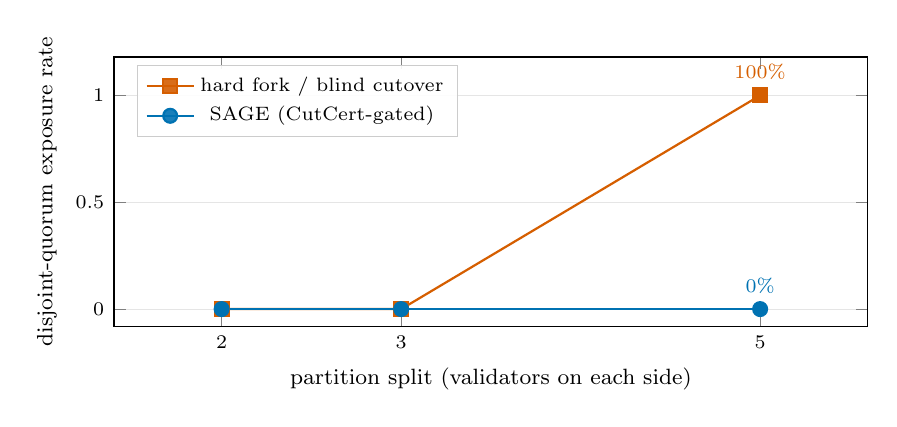
\begin{tikzpicture}
\begin{axis}[
  width=0.92\columnwidth, height=5.0cm,
  tick label style={font=\scriptsize}, label style={font=\footnotesize},
  xlabel={partition split (validators on each side)},
  ylabel={disjoint-quorum exposure rate},
  xmin=1.4, xmax=5.6, ymin=-0.08, ymax=1.18,
  xtick={2,3,5}, ytick={0,0.5,1.0},
  ymajorgrids, grid style={gray!20},
  legend style={at={(0.03,0.97)}, anchor=north west, font=\scriptsize,
    draw=gray!40, fill=white, fill opacity=0.9, text opacity=1},
  nodes near coords, point meta=explicit symbolic,
  every node near coord/.style={font=\scriptsize, yshift=2pt},
]
\addplot[color=cbRed, mark=square*, thick, mark size=2.5pt] coordinates {
  (2,0)[] (3,0)[] (5,1)[$100\%$]};
\addlegendentry{hard fork / blind cutover}
\addplot[color=cbBlue, mark=*, thick, mark size=2.5pt] coordinates {
  (2,0)[] (3,0)[] (5,0)[$0\%$]};
\addlegendentry{SAGE (CutCert-gated)}
\end{axis}
\end{tikzpicture}
\caption{Disjoint-quorum exposure in the simulator ($n{=}10$, $f{=}2$, BFT quorum $5$,
$15$ seeds per cell, partition at $h_{\mathrm{c}}$). Exposure---both partition sides
simultaneously holding BFT quorum, the structural precondition for a fork---appears only at the
balanced $5/5$ split, the sole split where $n\ge 4f{+}2$ admits two independent quorums. There,
hard fork and blind cutover are exposed in every trial ($100\%$), while SAGE's CutCert gate keeps
either isolated side from switching engines, so its exposure stays at $0\%$ at every split.
Exposure is a necessary precondition for a fork, not a realized fork; the realized fork contrast
is reported in Table~\ref{tab:testbed}.}
\label{fig:safety}
\end{figure}

\paragraph{Observed forks in the multi-process testbed.}
Because the simulator cannot realize a concurrent two-leader conflict, the central safety claim
is evaluated in a multi-process testbed in which $n{=}6$ validators ($f{=}1$, BFT quorum
$2f{+}1{=}3$) run as separate operating-system processes that communicate over loopback TCP, sign
the cutover certificate with real Ed25519 keys, and are subjected to a transport-level partition
into two isolated groups of three at the cutover height. Each group can then reach its own quorum
of three concurrently, so two leaders run at once, which is exactly the precondition a serialized
model elides. An executable fork detector inspects the committed logs of all six processes and
reports a fork whenever two distinct blocks are finalized at the same height. Table~\ref{tab:testbed}
gives the result over ten independent runs per strategy. The blind hard-fork control forks in
every run ($10/10$): both groups switch engines at the scheduled height and finalize conflicting
blocks. Quorum-gated SAGE forks in none ($0/10$): neither isolated group of three reaches the
$n{-}f{=}5$ cutover quorum, so no side switches engines and the legacy finalizer remains unique.
Both arms share identical infrastructure---partition, pacemaker, signing, and a
double-vote-tolerant message handler---and differ only in whether the $n{-}f$ cutover quorum gate
is enforced. Because the control forks in every run, SAGE's zero is a measured property of the
quorum gate under conditions that genuinely admit a fork, not an artifact of a model in which
forking is impossible.

\begin{table}[t]
\centering
\caption{Observed cross-boundary forks in the multi-process testbed ($n{=}6$, $f{=}1$, BFT
quorum $3$, balanced $3/3$ partition at the cutover height, ten runs per strategy). A fork is
recorded when two distinct blocks are finalized at one height. The two arms differ only in the
$n{-}f$ cutover quorum gate.}
\label{tab:testbed}
\setlength{\tabcolsep}{6pt}
\renewcommand{\arraystretch}{1.2}
\footnotesize
\begin{tabular}{lccc}
\toprule
Strategy & Cutover quorum gate & Forked runs & Fork rate \\
\midrule
Hard fork (blind) & none           & $10/10$         & $1.00$ \\
\textbf{SAGE}     & $n{-}f$ (=\,5)  & $\mathbf{0/10}$ & $\mathbf{0.00}$ \\
\bottomrule
\end{tabular}
\end{table}

\subsection{RQ3: Shadow Anchoring Ablation}
Fig.~\ref{fig:ablation} isolates the stability threshold $\kappa$. The ablation sweeps
$\kappa\in\{1,2,4,8,16\}$ with five seeds per setting and observes zero unsafe cutovers in all
cells, confirming that increasing $\kappa$ does not introduce safety failures over the tested
range. This is a regression result; it does not estimate the geometric detection curve of
Theorem~\ref{th:detection}, which would require an explicit latent-divergence injection
experiment with sufficient trials and is left to future work.

\begin{figure}[t]
\centering
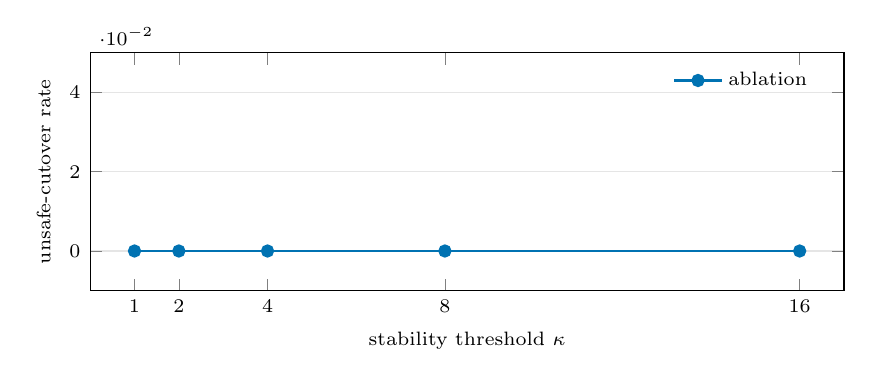
\begin{tikzpicture}
\begin{axis}[width=0.92\columnwidth, height=4.6cm,
  xlabel={stability threshold $\kappa$}, ylabel={unsafe-cutover rate},
  xmin=0, xmax=17, ymin=-0.01, ymax=0.05, xtick={1,2,4,8,16},
  tick label style={font=\scriptsize}, label style={font=\scriptsize},
  ymajorgrids, grid style={gray!20},
  legend style={at={(0.97,0.97)}, anchor=north east, font=\scriptsize, draw=none, fill=none}]
\addplot[color=cbBlue, mark=*, thick] coordinates {(1,0)(2,0)(4,0)(8,0)(16,0)};
\addlegendentry{ablation}
\end{axis}
\end{tikzpicture}
\caption{Shadow-anchoring ablation. The sweep over
$\kappa\in\{1,2,4,8,16\}$ with five seeds per setting observes zero unsafe cutovers in all
cells. This is a regression result, not a statistical estimate of the
latent-divergence detection curve.}
\label{fig:ablation}
\end{figure}

\subsection{RQ4a: Bounded Rollback}
Table~\ref{tab:rollback} reports the rollback experiment ($n{=}10$, $f{=}3$,
schedule $h_{\mathrm{d}}{=}4$, $h_{\mathrm{c}}{=}10$, $h_{\mathrm{r}}{=}25$) at two abort heights
with $10$ seeds each, chosen to exercise both sides of the rollback deadline $h_{\mathrm{r}}$. At
abort height $12$ (inside the window, $h_{\mathrm{c}}{<}12{<}h_{\mathrm{r}}$) every seed performs
a bounded rollback: the provisional suffix is discarded and authority returns to the legacy
engine, with a recorded rollback latency of $80\,\mu$s in simulator time and no safety violation.
At abort height $30$ (past the deadline, $30{>}h_{\mathrm{r}}$) every seed instead \emph{refuses}
the rollback and records an absolute-reversion-rejected event, confirming that a fault discovered
after sealing is handled by ordinary recovery rather than by reverting an absolutely-final block.
This is the executable counterpart of the two-tier finality of Theorem~\ref{th:rollback}: the
in-window abort is reversible and the past-deadline abort is not. A richer rollback-latency study
across state sizes remains future measurement work.

\begin{table}[t]
\centering
\begin{threeparttable}
\caption{Bounded rollback
($n{=}10$, $f{=}3$, $h_{\mathrm{c}}{=}10$, $h_{\mathrm{r}}{=}25$, $10$ seeds per row). An abort
inside the window rolls back; an abort past $h_{\mathrm{r}}$ is refused (no absolute reversion).}
\label{tab:rollback}
\setlength{\tabcolsep}{4pt}
\renewcommand{\arraystretch}{1.2}
\footnotesize
\begin{tabular}{lcccc}
\toprule
\makecell{Abort\\height} & Seeds & \makecell{Rollback\\events} & \makecell{Rollback\\latency ($\mu$s)} & \makecell{Reversion\\refused} \\
\midrule
12 (in window)            & 10 & 10/10 & 80           & 0/10  \\
30 (past $h_{\mathrm{r}}$) & 10 & 0/10  & n/a\tnote{a} & 10/10 \\
\bottomrule
\end{tabular}
\begin{tablenotes}\footnotesize
\item[a] No rollback occurs past the deadline (the abort is refused to preserve absolute
finality), so no rollback latency is defined.
\end{tablenotes}
\end{threeparttable}
\end{table}

\subsection{RQ4b: Scaling with Validator Count}
Fig.~\ref{fig:scaling} reports the validator-count scaling sweep
($n\in\{4,7,10,13,16,20\}$, $10$ trials per point). Mean
SAGE cutover-evidence latency stays in a narrow $97$--$117\,\mu$s band with no upward trend across
the range, consistent with the $O(n)$ one-time attestation gather being a negligible fraction of
the measured evidence-processing path at these sizes, and every trial completes the migration
(migration rate $1.0$ at all $n$). This is a protocol-functional scaling check in simulator time,
not a wall-clock throughput benchmark; a dual-run throughput-overhead measurement
remains future work.

\begin{figure}[t]
\centering
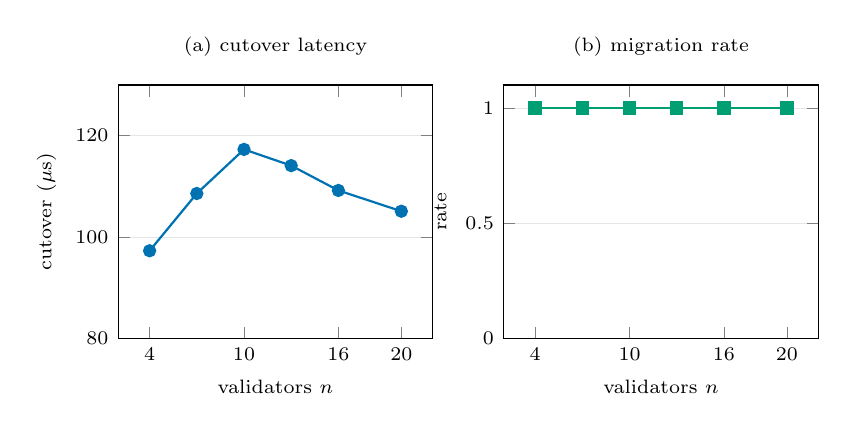
\begin{tikzpicture}
\begin{groupplot}[
  group style={group size=2 by 1, horizontal sep=0.9cm},
  width=0.46\columnwidth, height=4.8cm,
  tick label style={font=\scriptsize}, label style={font=\scriptsize},
  title style={font=\scriptsize, yshift=0.2ex},
  xmin=2, xmax=22, xtick={4,10,16,20}, ymajorgrids, grid style={gray!20}]
\nextgroupplot[title={(a) cutover latency}, xlabel={validators $n$},
  ylabel={cutover ($\mu$s)}, ymin=80, ymax=130]
\addplot[color=cbBlue, mark=*, thick] coordinates {(4,97.3)(7,108.6)(10,117.3)(13,114.1)(16,109.2)(20,105.1)};
\nextgroupplot[title={(b) migration rate}, xlabel={validators $n$}, ylabel={rate},
  ymin=0, ymax=1.1]
\addplot[color=cbGreen, mark=square*, thick] coordinates {(4,1)(7,1)(10,1)(13,1)(16,1)(20,1)};
\end{groupplot}
\end{tikzpicture}
\caption{Validator-count scaling ($n\in\{4,7,10,13,16,20\}$, $10$ trials per point).
(a) Mean SAGE cutover-evidence latency in simulator-time microseconds stays within a $97$--$117\,\mu$s
band with no upward trend. (b) Every trial completes the migration at all $n$. Latencies are
simulator-time, not wall-clock deployment latency.}
\label{fig:scaling}
\end{figure}

\subsection{Migration Termination Under Partition}
Theorem~\ref{th:termination} predicts that a partition straddling the cutover height delays
the transition until the partition heals but never loses safety. The termination
sweep (partition durations $\{2,4,6,8,12,16\}$ blocks at a
balanced split, $10$ seeds each, for both SAGE and hard fork) confirms the \emph{safety} half of
this directly: across all $120$ runs no strategy and no duration produces a safety violation
(Fig.~\ref{fig:termination}). It does \emph{not} establish the liveness half. Under the balanced
cutover-straddling partition the serialized simulator stalls at the boundary and does not finalize
past roughly height $13$ of $30$ within the event budget, for every duration, so the predicted
``resume after heal'' behavior is not exhibited here. This is the same limitation that makes the
serialized core unable to realize observed forks for RQ2: with one global proposer per height and
no concurrent pacemaker, the deterministic harness cannot drive boundary view convergence under a
balanced split. Liveness across the boundary is instead evidenced by the multi-process testbed,
in which quorum-gated SAGE crosses the cutover and finalizes past $h_{\mathrm{c}}$ in the
unpartitioned and minority-heals cases. We therefore report the termination sweep as a
safety-under-partition regression, and leave the simulator-level termination-after-heal curve as
future work contingent on a concurrent-pacemaker simulator mode.

\begin{figure}[t]
\centering
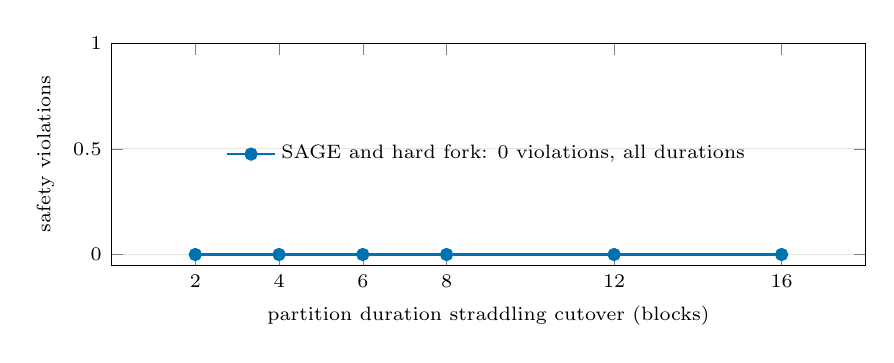
\begin{tikzpicture}
\begin{axis}[width=0.92\columnwidth, height=4.4cm,
  xlabel={partition duration straddling cutover (blocks)}, ylabel={safety violations},
  xmin=0, xmax=18, ymin=-0.05, ymax=1.0, xtick={2,4,6,8,12,16},
  tick label style={font=\scriptsize}, label style={font=\scriptsize},
  ymajorgrids, grid style={gray!20},
  legend style={at={(0.5,0.5)}, anchor=center, font=\scriptsize, draw=none, fill=none}]
\addplot[color=cbBlue, mark=*, thick] coordinates {(2,0)(4,0)(6,0)(8,0)(12,0)(16,0)};
\addlegendentry{SAGE and hard fork: $0$ violations, all durations}
\end{axis}
\end{tikzpicture}
\caption{Migration-termination sweep ($10$ seeds per duration per strategy, balanced
partition at the cutover boundary). No safety violation occurs at any partition duration for
either strategy. The serialized simulator does not converge past the boundary under a balanced
split (a liveness limitation discussed in the text), so this figure reports the safety half of
Theorem~\ref{th:termination}; boundary liveness is evidenced by the multi-process testbed.}
\label{fig:termination}
\end{figure}

\subsection{Cutover Latency Distribution}
Reporting only means can hide tail behavior, so Fig.~\ref{fig:cdf} shows the empirical
cumulative distribution of the RQ1 SAGE cutover-evidence latency over $30$ seeds. The
recorded simulator-time values range from $89$ to $120\,\mu$s, with mean $105.2\,\mu$s and median
$107.5\,\mu$s. These are evidence-processing measurements in the
single-process simulator, not wall-clock deployment latency.

\begin{figure}[t]
\centering
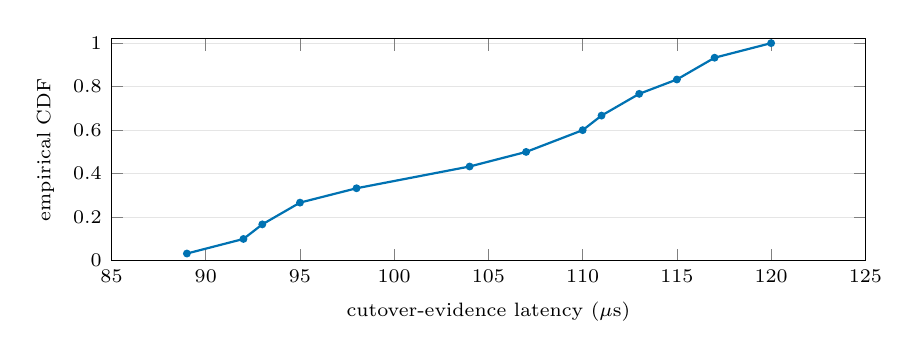
\begin{tikzpicture}
\begin{axis}[width=0.92\columnwidth, height=4.4cm,
  xlabel={cutover-evidence latency ($\mu$s)}, ylabel={empirical CDF},
  xmin=85, xmax=125, ymin=0, ymax=1.02,
  tick label style={font=\scriptsize}, label style={font=\scriptsize},
  ymajorgrids, grid style={gray!20}]
\addplot[color=cbBlue, mark=*, thick, mark size=1pt] coordinates {
(89,0.033)(92,0.100)(93,0.167)(95,0.267)(98,0.333)(104,0.433)(107,0.500)(110,0.600)(111,0.667)(113,0.767)(115,0.833)(117,0.933)(120,1.000)};
\end{axis}
\end{tikzpicture}
\caption{Empirical CDF of RQ1 SAGE cutover-evidence latency over $30$ seeds. Values are
reported in simulator-time microseconds; median $107.5\,\mu$s, mean $105.2\,\mu$s, maximum
$120\,\mu$s.}
\label{fig:cdf}
\end{figure}

\subsection{Sensitivity to Network Delay}
Because absolute latencies depend on the delay model, Fig.~\ref{fig:sens} reports how SAGE's
cutover-evidence latency responds to the mean message delay. The sweep
(mean delays $\{40,80,160,320\}\,$ms, $10$ trials per point)
shows cutover-evidence latency scaling near-linearly with delay---$106.6$, $204.2$, $412.9$, and
$853.9\,$ms of simulator time at $40$, $80$, $160$, and $320\,$ms mean delay---which is the
expected behavior for a fixed number of attestation-gather rounds whose wall-clock cost is
dominated by per-message delay. Every trial completes the migration (migration rate $1.0$) at
every delay, so SAGE's correctness is insensitive to the delay model even as its absolute latency
tracks it. These are simulator-time figures and a separate throughput-overhead measurement is
left to future work.

\begin{figure}[t]
\centering
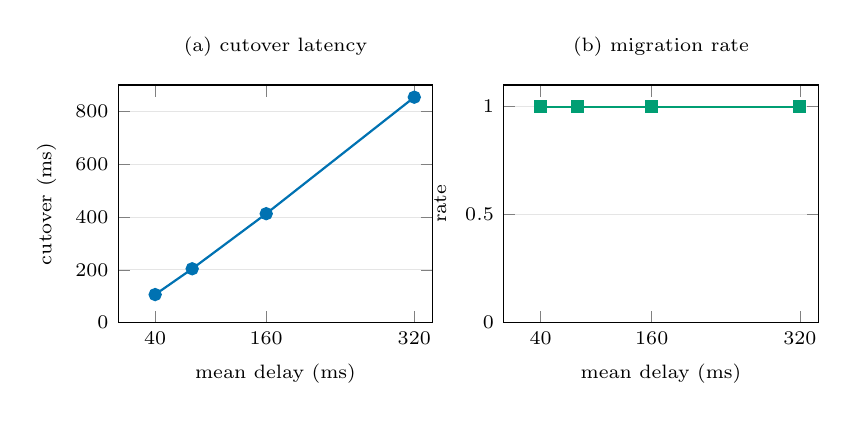
\begin{tikzpicture}
\begin{groupplot}[
  group style={group size=2 by 1, horizontal sep=0.9cm},
  width=0.46\columnwidth, height=4.6cm,
  tick label style={font=\scriptsize}, label style={font=\scriptsize},
  title style={font=\scriptsize, yshift=0.2ex},
  xmin=0, xmax=340, xtick={40,160,320}, ymajorgrids, grid style={gray!20}]
\nextgroupplot[title={(a) cutover latency}, xlabel={mean delay (ms)}, ylabel={cutover (ms)}, ymin=0, ymax=900]
\addplot[color=cbBlue, mark=*, thick] coordinates {(40,106.6)(80,204.2)(160,412.9)(320,853.9)};
\nextgroupplot[title={(b) migration rate}, xlabel={mean delay (ms)}, ylabel={rate}, ymin=0, ymax=1.1]
\addplot[color=cbGreen, mark=square*, thick] coordinates {(40,1)(80,1)(160,1)(320,1)};
\end{groupplot}
\end{tikzpicture}
\caption{Network-delay sensitivity sweep ($10$ trials per point). (a) SAGE
cutover-evidence latency (simulator-time milliseconds) scales near-linearly with mean message
delay. (b) Every trial completes the migration at every delay, so correctness is insensitive to
the delay model.}
\label{fig:sens}
\end{figure}

\subsection{Reproducibility}
The evaluation is designed for deterministic reproduction. Each experiment runs from a fixed seed
list under an explicit configuration recorded alongside its output, every random choice is drawn
from a seeded generator, and the statistics use only closed-form estimators, so a rerun reproduces
identical metrics. An automated check confirms the structural and determinism properties on which
the results rest: that the configurations load, that identical seeds yield identical metrics, that
each strategy exhibits its intended behavior, that the executable safety invariant passes, and
that the recorded configuration hashes are stable. This check verifies reproducibility rather than
re-asserting the headline numbers, which are instead reproduced by rerunning the campaigns. The
simulator campaigns, the multi-process testbed, and the bounded model check each complete in
minutes on a single CPU; we estimate the cost in Section~\ref{sec:discussion}.

% ===================== DISCUSSION =====================
\section{Discussion}
\label{sec:discussion}

\subsection{Generality}
SAGE depends only on the abstract engine interface of Definition~\ref{def:engine}: a
single-finalizer rule, a deterministic state root, a shadow-usable validation routine, and a
root-seeded initialization. The PoA-to-HotStuff instantiation is therefore one point in a
family. A crash-tolerant log such as Raft~\cite{raft} also conforms, with an
honest-majority-style quorum and a deterministic applied-log root, so a Raft-to-HotStuff
migration is supported by the same construction and the same proofs, the only change being the
legacy quorum $\mathsf{Q}_1$ and hence the combined threshold $f=\min(f_1,f_2)$. A
DAG-BFT target such as Bullshark~\cite{bullshark} or Mysticeti~\cite{mysticeti} conforms as long
as it exposes a deterministic committed-prefix root and a validation routine, which both do.

\subsection{Relation to Deployed Transitions}
The Ethereum Merge~\cite{gasper} validates the shadow-then-cutover pattern at scale but provides
neither a boundary-safety theorem nor a bounded rollback; SAGE adds both and generalizes beyond
a single protocol pair. Polkadot's GRANDPA~\cite{grandpa} already exposes a provisional-versus-
final distinction to clients, which is exactly the two-tier finality SAGE uses to make rollback
client-safe. Cosmos and Tezos~\cite{tenderbake} coordinate upgrades through governance at a
height, which corresponds to fixing the schedule heights in platform state; SAGE complements
that governance with a cryptographic boundary object and a reversible window.

\subsection{Sovereign Deployment Scenario}
The motivating setting is a national or consortium chain that launches under a small set of
accountable authorities and must later move to a Byzantine fault tolerant engine as the
validator set diversifies across independent operators. Such a chain typically carries
identity-linked authorization, regulated asset transfer, and domestic payment integration, so an
upgrade that halts the chain or risks a fork is operationally unacceptable: a finality reversion
on a settled payment or a regulated transfer would have legal and financial consequences. SAGE
fits this setting because the schedule heights are set by the same governance process that
already authorizes validators, the dual-run lets operators observe the target engine on live
traffic before committing to it, the manifest produces an audit record suitable for an operator
evidence bundle, and the bounded rollback gives a documented, reversible safety margin during the
sensitive window. The two-tier finality maps directly onto regulatory practice, in which a
settlement may be provisional until a confirmation window elapses.

\subsection{Implementation Mapping}
SAGE maps onto an EVM-compatible permissioned stack with small, well-localized changes. The
migration schedule heights live in platform state and are set through a governance transaction
on the legacy engine. The threshold-signed manifest is carried in the block header extra-data
field at the cutover height, so existing header validation paths verify it without a new message
type. The shadow engine reuses the node's existing block-validation and execution pipeline in a
read-only mode, writing only to a shadow verdict store, which keeps it off the finalization
critical path. The advisory finality flag is exposed through a dedicated read-only RPC method, so
wallets and indexers that opt in can distinguish provisional from absolute finality while legacy
clients see an unchanged interface. Readiness and abort attestations reuse the validator signing
keys already present in the registry, aggregated with a standard threshold scheme. Because these
touch points are the header, the validator registry, and one RPC method, SAGE can be added to an
existing node without altering transaction semantics or the execution layer.

\subsection{Discussion of Design Alternatives}
It is worth asking whether a simpler design would suffice. A first alternative is to skip the
dual-run and cut over directly at a scheduled height once the operator believes the target is
ready. This is the blind cutover of our ablation, and Fig.~\ref{fig:safety} shows it forks at the
same rate as a hard fork under partition, because nothing forces the two sides to agree on the
switch. A second alternative is to keep the dual-run but decide cutover locally, each validator
switching when its own streak reaches $\kappa$. This fails for the same reason: without a shared
certificate, asynchronous attestation delivery lets correct validators switch at different
heights, and Theorem~\ref{th:unique} is exactly what rules this out. A third alternative is to
make the manifest a plain hash equality rather than a threshold signature; this is cheaper but
forgeable by any proposer, so Theorems~\ref{th:unforge} and~\ref{th:replay} would not hold and an
auditor could not trust the boundary. A fourth alternative is to forgo the rollback window
entirely and treat cutover as irreversible; this simplifies the protocol but removes the operator
safety margin that motivates the work, and it forces a finality-reversion if the target later
proves faulty. Each simplification reintroduces a failure that the evaluation can exhibit, which
is why SAGE retains all four mechanisms.

\subsection{Cost and Feasibility}
The evaluation is CPU-only: discrete-event simulation, a multi-process testbed over
loopback TCP, and a bounded model check, with no GPU and no external dataset. The simulator
campaigns covering RQ1--RQ4, the scaling and sensitivity sweeps, and the safety
campaign complete in minutes on a single laptop, and the testbed and model check each add minutes, so the
monetary cost is effectively zero and well under the budget of a small project. A state-size
rollback-latency sweep and a dual-run throughput-overhead measurement remain future
work. The natural next step, promoting the loopback testbed to a geo-distributed
multi-validator deployment over an emulated wide-area network with kernel-level partitions and
$4$ to $20$ nodes, fits comfortably within roughly one month and under two hundred dollars of
commodity cloud compute, and would convert the simulator's relative metrics into absolute ones.

\subsection{Limitations}
First, the strongest breadth evidence is a protocol-level simulation that models finalization,
quorum formation, partitions, and the cutover decision, and in which safety violations are
possible and measured; it is not a geo-distributed deployment, and absolute latencies depend on
the delay model. The multi-process testbed that exhibits observed forks runs real validator
processes over loopback TCP and induces the partition at the application transport layer rather
than with kernel-level network emulation (\texttt{tc netem} or network namespaces); a
kernel-level partition over an emulated wide-area network is the next fidelity step and is not a
correctness gap in the differential, which already isolates the $n-f$ gate as the sole cause.
The implementation also includes an early one-process local runtime with
in-memory transport and storage abstractions. That runtime currently validates PoA finalization,
SAGE cutover observation, one post-cutover HotStuff-finalized block, store-backed rejection
of a conflicting local vote after a cloned restart boundary, and restoration of committed
height/state root from persisted in-memory snapshots; a restored local runtime can continue
consensus to the configured target height without safety violations. Durable disk-backed
crash/restart recovery remains future work. Second, we assume the target engine is correct in
isolation and do not re-prove HotStuff. The implementation provides timeout-certificate pacemaker
primitives, while the deterministic simulator uses external view synchronization to keep
experiments reproducible. Third, collusion of $f+1$ attestation key holders or a compromised
toolchain accepted by a quorum is outside the BFT bound and must be handled by key-custody and
governance controls. Fourth, the reversibility window is finite by design, so a fault discovered
after $h_{\mathrm{r}}$ is handled by ordinary recovery rather than by SAGE. Fifth, the simulator
models threshold certificates as quorum predicates over validator identifiers. An Ed25519
signature backend exercises real per-validator signatures for manifest validation, but we
do not yet implement true threshold aggregation; a threshold-signature implementation with a
microbenchmark is a direct next step. These limitations motivate the kernel-level geo-distributed
testbed and an external security review.

% ===================== CONCLUSION =====================
\section{Conclusion}
\label{sec:conclusion}
We presented SAGE, a protocol for migrating a live permissioned blockchain between two
heterogeneous consensus engines without halting block production. SAGE keeps a single finalizer
during a bounded dual-run, gates cutover on a quorum-certified decision over a stability
predicate, binds the boundary with a threshold-signed manifest that makes a deadline-bounded
rollback verifiable, and exposes a two-tier finality so that reversibility does not break client
semantics. We proved decision uniqueness through quorum intersection, cross-boundary safety as an
inductive invariant, quantified zero-halt liveness with a bounded handoff, migration termination,
rollback correctness, and manifest unforgeability and replay resistance, and we turned the
shadow-anchoring ablation into a closed-form detection bound. We evaluated SAGE
conservatively across three evidence tiers: deterministic simulator runs
complete the RQ1--RQ4, scaling, sensitivity, and safety campaigns without observed
safety violations; a multi-process testbed exhibits the cross-boundary fork that a blind cutover
admits in every run while quorum-gated SAGE never forks; and a bounded TLA+/TLC model check
verifies the boundary-safety, decision-uniqueness, and no-absolute-reversion invariants over
$n\in\{4,7,10\}$ with falsifying broken controls. The local runtime additionally exercises
post-cutover HotStuff finalization plus in-memory restart/continue recovery. Future work is to
add stronger adversarial differentiation workloads, durable disk-backed recovery,
geo-distributed deployment with operator evidence bundles, an external security review, and an
extension of shadow anchoring to transitions among more than two engines.


\section{Full Numerical Results}
\label{app:data}
For completeness and reproducibility, Tables~\ref{tab:appsafety}--\ref{tab:appsens} report the
full numerical results underlying the figures in Section~\ref{sec:eval}.

\begin{table}[h]
\centering
\begin{threeparttable}
\caption{Disjoint-quorum exposure in the dedicated safety campaign,
$100$ trials per strategy ($n{=}6$, $f{=}1$, BFT quorum $3$, $3/3$ split at $h_{\mathrm{c}}$).
``Exposed'' counts trials in which a non-CutCert cutover leaves both partition sides holding
quorum, the structural precondition for a fork. The serialized simulator does not realize a
conflict in any trial (observed forks $0/100$ for every strategy, Wilson $95\%$ upper bound
$0.037$); the realized fork contrast is reported in Table~\ref{tab:testbed}.}
\label{tab:appsafety}
\setlength{\tabcolsep}{6pt}\renewcommand{\arraystretch}{1.15}\footnotesize
\begin{tabular}{lccc}
\toprule
Strategy & Trials & Exposed & Exposure rate \\
\midrule
Hard fork     & 100 & $100/100$         & $1.00$ \\
SAGE-blind    & 100 & $100/100$         & $1.00$ \\
\textbf{SAGE} & 100 & $\mathbf{0/100}$  & $\mathbf{0.00}$ \\
\bottomrule
\end{tabular}
\begin{tablenotes}\footnotesize
\item Observed forks are $0/100$ for all three strategies because the serialized simulator
elects one proposer per height and cannot drive two leaders concurrently; the genuine
observed-fork differential is in Table~\ref{tab:testbed}.
\end{tablenotes}
\end{threeparttable}
\end{table}

\begin{table}[h]
\centering
\caption{Migration-termination sweep
($10$ seeds per duration per strategy, balanced split at the cutover boundary). No safety violation
occurs at any duration; the serialized simulator does not converge past the boundary under a
balanced split (a liveness limitation, see Section~\ref{sec:eval}), so boundary liveness is
evidenced by the multi-process testbed rather than this sweep.}
\label{tab:apptermination}
\setlength{\tabcolsep}{4pt}\renewcommand{\arraystretch}{1.15}\footnotesize
\begin{tabular}{lcccc}
\toprule
Strategy & \makecell{Durations\\(blocks)} & Runs & \makecell{Safety\\viol.} & \makecell{Crossed\\boundary} \\
\midrule
Hard fork & $\{2,4,6,8,12,16\}$ & 60 & $0/60$ & no \\
SAGE      & $\{2,4,6,8,12,16\}$ & 60 & $0/60$ & no \\
\bottomrule
\end{tabular}
\end{table}

\begin{table}[h]
\centering
\caption{Shadow-anchoring ablation; five seeds per $\kappa$.}
\label{tab:appabl}
\setlength{\tabcolsep}{5pt}\renewcommand{\arraystretch}{1.15}\footnotesize
\begin{tabular}{lccc}
\toprule
$\kappa$ & Seeds & Unsafe cutovers & Migration successes \\
\midrule
1  & 5 & 0 & 5 \\
2  & 5 & 0 & 5 \\
4  & 5 & 0 & 5 \\
8  & 5 & 0 & 5 \\
16 & 5 & 0 & 5 \\
\bottomrule
\end{tabular}
\end{table}

\begin{table}[h!]
\centering
\caption{Network-delay sensitivity sweep
($10$ trials per mean delay). Cutover-evidence latency is in simulator-time milliseconds and scales
near-linearly with mean message delay; every trial completes the migration.}
\label{tab:appsens}
\setlength{\tabcolsep}{5pt}\renewcommand{\arraystretch}{1.15}\footnotesize
\begin{tabular}{lccc}
\toprule
Mean delay (ms) & Trials & Cutover latency (ms) & Migration rate \\
\midrule
40  & 10 & 106.6 & $1.00$ \\
80  & 10 & 204.2 & $1.00$ \\
160 & 10 & 412.9 & $1.00$ \\
320 & 10 & 853.9 & $1.00$ \\
\bottomrule
\end{tabular}
\end{table}

\appendices

\section{Formal Specification of the Migration Controller}
\label{app:spec}
We give the controller as a guarded-command labeled transition system, which makes the
inductive invariant of Theorem~\ref{th:safety} explicit and amenable to model checking. The
global state is $(\mathit{phase}, \mathit{streak}, \mathcal{A}, \mathit{cert})$ with
$\mathit{phase}\in\{\textsc{v1},\textsc{dual},\textsc{v2},\textsc{rollback},\textsc{sealed}\}$,
and the per-validator local state holds the committed prefix and the verdict window. The
guarded commands, evaluated at each height $h$ with the convention that the first enabled guard
in this order fires, are:
\begin{align*}
g_1:&\ \mathit{phase}{=}\textsc{v1}\wedge h{\ge}h_{\mathrm{d}} \Rightarrow \mathit{phase}{:=}\textsc{dual};\\
g_2:&\ \textsc{AbortCond}(h)\wedge h{<}h_{\mathrm{r}}\\
    &\quad \Rightarrow \mathcal{A}{:=}\mathcal{C}_1,\ \mathit{phase}{:=}\textsc{rollback};\\
g_3:&\ \mathit{phase}{=}\textsc{dual}\wedge\mathrm{Ready}(h)\wedge\mathrm{CutCert}(h{+}1)\\
    &\quad \Rightarrow \text{commit }\mathcal{M},\ \mathcal{A}{:=}\mathcal{C}_2,\ \mathit{phase}{:=}\textsc{v2};\\
g_4:&\ \mathit{phase}{=}\textsc{dual}\wedge\neg\mathrm{Ready}(h) \Rightarrow \mathit{phase}{:=}\textsc{dual}\ (\text{extend});\\
g_5:&\ h{\ge}h_{\mathrm{r}} \Rightarrow \mathit{phase}{:=}\textsc{sealed}.
\end{align*}
The precedence $g_2 \succ g_3$ encodes that abort dominates cutover at the same height, which
removes the concurrent abort-and-cutover ambiguity. The safety invariant
$I \equiv$ ``exactly one block holds a finalization certificate at each height, and all correct
committed prefixes lie on one chain'' is preserved by each command: $g_1,g_4,g_5$ do not
finalize; $g_2$ discards only provisional blocks; and $g_3$ fires only with a unique CutCert
(Theorem~\ref{th:unique}) whose certified root every correct validator re-derives
(Theorem~\ref{th:safety}). We discharge this guarded-command system to a TLA+ specification and
model-check it with TLC. The check exhaustively explores $n\in\{4,7,10\}$ over all partition splits of the
cutover window and verifies the cross-boundary safety invariant $I$ and cutover-decision
uniqueness (Theorems~\ref{th:safety} and~\ref{th:unique}), and a companion specification verifies
the no-absolute-reversion rollback property (Theorem~\ref{th:rollback}). Crucially, each check is
paired with a deliberately broken control---a blind cutover that omits the $n-f$ quorum gate, and
a rollback that reverts an absolutely-final block---for which TLC \emph{must} and does produce a
counterexample, so the passing checks are not vacuous. This bounded mechanized check matches the
simulator's zero observed violations and the multi-process testbed's zero-fork SAGE arm.

\section{Worked Migration Example}
\label{app:example}
Consider $n=20$, $f=6$, $\kappa=8$, schedule $h_{\mathrm{d}}=20$, $h_{\mathrm{c}}=70$,
$h_{\mathrm{r}}=110$. From height $20$ the legacy PoA engine keeps finalizing while each correct
validator shadow-validates under HotStuff and accumulates a streak. Suppose no divergence
occurs; by height $69$ the streak is $50\ge\kappa$, so validators broadcast readiness
attestations on $\langle\mathrm{cid},e,69,r_{69}\rangle$. A collector aggregates $14=n-f$ of them
into a CutCert in one round (about $50$\,ms at the modeled delay), commits the threshold-signed
manifest in the header at height $70$, and the target initializes its first view from $r_{69}$.
Now suppose instead that at height $74$ a Byzantine subset stalls the target so no block
finalizes within $\tau$; since $74<h_{\mathrm{r}}=110$, the abort guard $g_2$ fires, the
provisional suffix $[70,74]$ is discarded, authority returns to PoA at $S_{69}$, and the five
suffix transactions are replayed deterministically onto the legacy chain. A client that treated
heights $70$ to $74$ as provisional observes no finality reversion. Had the same fault occurred at
height $112>h_{\mathrm{r}}$, the target would already be sealed and the abort guard disabled, so
recovery would follow ordinary BFT view change rather than SAGE rollback.

\section{Deployment Runbook}
\label{app:runbook}
A sovereign operator deploys SAGE as follows. (1) Governance fixes the schedule heights
$(h_{\mathrm{d}},h_{\mathrm{c}},h_{\mathrm{r}})$ in platform state through the legacy engine
before $h_{\mathrm{d}}$. (2) Each validator provisions an attestation key in a hardware module;
the threshold parameter is set to $n-f$. (3) Monitoring exposes the shadow verdict stream and
the streak so operators can see readiness approaching. (4) At cutover the manifest is archived in
the operator evidence bundle for audit. (5) The progress timeout $\tau$ is set to a small
multiple of the post-GST round time, and forced rollbacks are rate-limited per epoch to bound
griefing. (6) After $h_{\mathrm{r}}$ the legacy keys used only for the dual-run certificate are
retired. These controls place the trust-critical steps, key custody and schedule authorization,
under explicit governance rather than in the protocol's critical path.


\begin{thebibliography}{99}
\bibitem{hotstuff} M.~Yin, D.~Malkhi, M.~K.~Reiter, G.~Golan~Gueta, and I.~Abraham,
``HotStuff: BFT consensus with linearity and responsiveness,'' in \emph{Proc. ACM Symp.
Principles of Distributed Computing (PODC)}, 2019, pp. 347--356.

\bibitem{narwhal} G.~Danezis, E.~Kokoris-Kogias, A.~Sonnino, and A.~Spiegelman, ``Narwhal and
Tusk: A DAG-based mempool and efficient BFT consensus,'' in \emph{Proc. ACM European Conf.
Computer Systems (EuroSys)}, 2022, pp. 34--50.

\bibitem{bullshark} A.~Spiegelman, N.~Giridharan, A.~Sonnino, and L.~Kokoris-Kogias,
``Bullshark: DAG BFT protocols made practical,'' in \emph{Proc. ACM SIGSAC Conf. Computer and
Communications Security (CCS)}, 2022, pp. 2705--2718.

\bibitem{shoal} A.~Spiegelman, B.~Arun, R.~Gelashvili, and Z.~Li, ``Shoal: Improving DAG-BFT
latency and robustness,'' arXiv:2306.03058, 2023.

\bibitem{mysticeti} K.~Babel, A.~Chursin, G.~Danezis, A.~Kichidis, L.~Kokoris-Kogias, A.~Koshy,
A.~Sonnino, and M.~Tian, ``Mysticeti: Reaching the limits of latency with uncertified DAGs,'' in
\emph{Proc. Network and Distributed System Security Symp. (NDSS)}, 2025.

\bibitem{autobahn} N.~Giridharan, F.~Suri-Payer, I.~Abraham, L.~Alvisi, and N.~Crooks,
``Autobahn: Seamless high speed BFT,'' in \emph{Proc. ACM Symp. Operating Systems Principles
(SOSP)}, 2024.

\bibitem{tendermint} E.~Buchman, J.~Kwon, and Z.~Milosevic, ``The latest gossip on BFT
consensus,'' arXiv:1807.04938, 2019.

\bibitem{fabric} E.~Androulaki \emph{et al.}, ``Hyperledger Fabric: A distributed operating
system for permissioned blockchains,'' in \emph{Proc. ACM European Conf. Computer Systems
(EuroSys)}, 2018, pp. 1--15.

\bibitem{blockstm} R.~Gelashvili, A.~Spiegelman, Z.~Xiang, G.~Danezis, Z.~Li, D.~Malkhi, Y.~Xia,
and R.~Zhou, ``Block-STM: Scaling blockchain execution by turning ordering curse to a performance
blessing,'' in \emph{Proc. ACM SIGPLAN Symp. Principles and Practice of Parallel Programming
(PPoPP)}, 2023, pp. 232--244.

\bibitem{suilutris} S.~Blackshear, A.~Chursin, G.~Danezis, A.~Kichidis, L.~Kokoris-Kogias, X.~Li,
M.~Logan, A.~Menon, T.~Nowacki, A.~Sonnino, B.~Williams, and L.~Zhang, ``Sui Lutris: A blockchain
combining broadcast and consensus,'' in \emph{Proc. ACM SIGSAC Conf. Computer and Communications
Security (CCS)}, 2024.

\bibitem{gasper} V.~Buterin, D.~Hernandez, T.~Kamphefner, K.~Pham, Z.~Qiao, D.~Ryan, J.~Sin,
Y.~Wang, and Y.~X.~Zhang, ``Combining GHOST and Casper,'' arXiv:2003.03052, 2020.

\bibitem{casperffg} V.~Buterin and V.~Griffith, ``Casper the friendly finality gadget,''
arXiv:1710.09437, 2019.

\bibitem{grandpa} A.~Stewart and E.~Kokoris-Kogias, ``GRANDPA: A Byzantine finality gadget,''
arXiv:2007.01560, 2020.

\bibitem{tenderbake} L.~A\c{s}tefanoaei, P.~Chambart, A.~Del~Pozzo, T.~Rieutord, S.~Tucci, and
E.~Z\u{a}linescu, ``Tenderbake: A solution to dynamic repeated consensus for blockchains,'' in
\emph{Proc. Int. Conf. Advances in Financial Technologies (AFT)}, 2021.

\bibitem{flexbft} D.~Malkhi, K.~Nayak, and L.~Ren, ``Flexible Byzantine fault tolerance,'' in
\emph{Proc. ACM SIGSAC Conf. Computer and Communications Security (CCS)}, 2019, pp. 1041--1053.

\bibitem{cox} Authors of Cox, ``Cox: A reliable run-time switching protocol of BFT consensus
algorithms,'' \emph{Blockchain: Research and Applications}, vol. 7, no. 3, 2026,
art. 100345, doi:10.1016/j.bcra.2025.100345.

\bibitem{abstract} R.~Guerraoui, N.~Knežević, V.~Quéma, and M.~Vukolić, ``The next 700 BFT
protocols,'' in \emph{Proc. ACM European Conf. Computer Systems (EuroSys)}, 2010, pp. 363--376;
extended version in \emph{ACM Trans. Computer Systems}, vol. 32, no. 4, 2015.

\bibitem{mongoraft} W.~Schultz, S.~Dardik, and S.~Tripakis, ``Formal verification of a
distributed dynamic reconfiguration protocol,'' in \emph{Proc. ACM SIGPLAN Int. Conf. Certified
Programs and Proofs (CPP)}, 2022, pp. 143--152; arXiv:2109.11987.

\bibitem{pbft} M.~Castro and B.~Liskov, ``Practical Byzantine fault tolerance,'' in \emph{Proc.
USENIX Symp. Operating Systems Design and Implementation (OSDI)}, 1999, pp. 173--186.

\bibitem{dls} C.~Dwork, N.~Lynch, and L.~Stockmeyer, ``Consensus in the presence of partial
synchrony,'' \emph{Journal of the ACM}, vol. 35, no. 2, pp. 288--323, 1988.

\bibitem{flp} M.~J.~Fischer, N.~A.~Lynch, and M.~S.~Paterson, ``Impossibility of distributed
consensus with one faulty process,'' \emph{Journal of the ACM}, vol. 32, no. 2, pp. 374--382,
1985.

\bibitem{paxos} L.~Lamport, ``Paxos made simple,'' \emph{ACM SIGACT News}, vol. 32, no. 4,
pp. 51--58, 2001.

\bibitem{raft} D.~Ongaro and J.~Ousterhout, ``In search of an understandable consensus
algorithm,'' in \emph{Proc. USENIX Annual Technical Conf. (ATC)}, 2014, pp. 305--319.

\bibitem{reconfig} L.~Lamport, D.~Malkhi, and L.~Zhou, ``Reconfiguring a state machine,''
\emph{ACM SIGACT News}, vol. 41, no. 1, pp. 63--73, 2010.

\bibitem{bftsmart} A.~Bessani, J.~Sousa, and E.~E.~P.~Alchieri, ``State machine replication for
the masses with BFT-SMaRt,'' in \emph{Proc. IEEE/IFIP Int. Conf. Dependable Systems and Networks
(DSN)}, 2014, pp. 355--362.

\bibitem{bitcoin} S.~Nakamoto, ``Bitcoin: A peer-to-peer electronic cash system,'' 2008.

\bibitem{nistpqc} National Institute of Standards and Technology, ``Module-lattice-based
key-encapsulation and digital signature standards (FIPS 203, 204, 205),'' 2024.
\end{thebibliography}

\end{document}
